\fancychapter{Minimal models of electron correlations in energy bands}
\label{cap:hubbard}

\slshape

We start with an overview of the Hubbard model and in the following chapters we provide details on how to simulate it numerically using Quantum Monte Carlo. We discuss the original motivation provided by Hubbard to introduce the model and show how its Hamiltonian arises as an approximate representation of the Coulomb repulsion between electrons in an energy band. Then, we present exact solutions for particular limiting cases, which are used to crosscheck our simulations. In particular, we show that, in the limit where the interaction is large, the effective Hamiltonian at half filling corresponds to an atomic Heisenberg model defined in the appropriate Hilbert space with one electron per site.
Then, we introduce Green's functions and explain how they relate to Wick's theorem. We proceed by formulating the mean field theory of the Hubbard model, and comparing results for a \acs{1D} chain with those obtained from Stoner's criterion.
Finally, we show how one can generalize the Hubbard Hamiltonian and finish by discussing what type of interaction terms may be recast in a way that is more prone to simulation.

\normalfont

\section{Modelling electron correlations}\label{sec:intro}

The Hubbard model appeared in 1963 as one of the first attempts to include electron interaction effects in a quantum mechanical description of a solid.
Originally, it was introduced to explain the behavior of the electrons in the narrow, partially filled $d-$bands of transition metals \cite{hubbard_electron_1963}.
Correlation phenomena due to the Coulomb repulsion between the electrons in these bands lead to a behavior reminiscent of the atomic picture of a solid.
In fact, the model may simply be regarded as a minimal model of interacting electrons in an energy band of a solid, where only on-site interactions are considered.
We have come a long way since the introduction of the Hubbard model and it is now arguably as paradigm-defining in many-body theory as the Ising model in statistical physics \cite{fazekas_lecture_1999, mahan_many-particle_2000, altland_condensed_2010}.

Although the Hubbard model was initially applied to transition metal monoxides like \chem{FeO}, \chem{NiO}, and \chem{CoO}, which are antiferromagnetic insulators (and not metallic, as was initially thought)\footnote{They were predicted to be metals by band theory until they were found not to behave like metals empirically.}, it is a minimal model giving insight on insulating, magnetic, and even superconducting phases arising due to the effect of electron interactions in a variety of quantum systems.

\begin{figure}[H]
	\centering
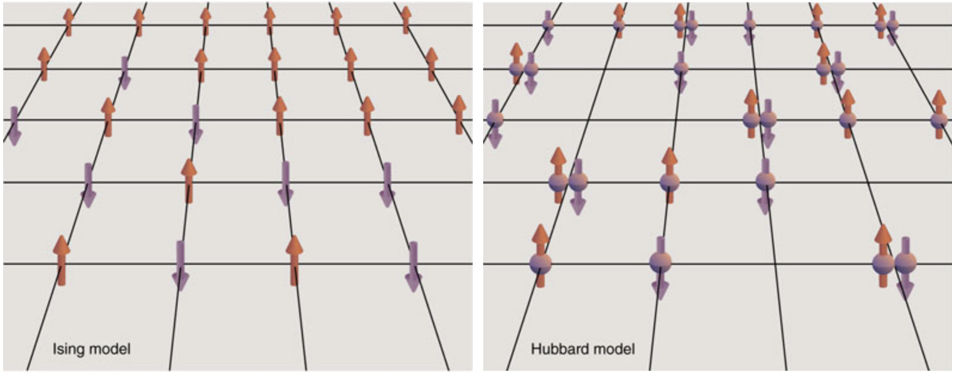
\includegraphics[width=0.9\linewidth]{Hubbard/IsingVsHubbard.jpeg}
	\caption[Graphical comparison between the Ising and the Hubbard models.]{Unlike the Ising model, where either an up or a down spin live at each site, in the Hubbard model, there are four possible states at each site: a "hole" (absence of an electron), either an up spin electron or a down spin electron, or two electrons of opposite spins.
	The idea behind the model is to consider that the electrons interact, repelling each other, only when they are on the same site (taken from \cite{hayes_hip-hop_2009}).}
	\label{fig:IsingVsHubbard}
\end{figure}

Of course, Figure (\ref{fig:IsingVsHubbard}) is only a simplified view presented for the sake of analogy.
The Hubbard model is actually defined in terms of a Hamiltonian acting on electron wave functions centered in the sites of a lattice.
Ultimately, we wish to determine, or at least approximate, the wave function describing the full electronic system.
To do so, we must consider a Hamiltonian that allows simultaneous charge and spin fluctuations.
It turns out that the \emph{many-body} wave function we seek is not, in general, a simple combination of products of one electron wave functions, as in the interaction-free case.

When Hubbard's seminal paper came out, it followed a trend that arose in the 1950's when people were working on a theory of correlation effects in the free electron gas \cite{bohm_collective_1953, gell-mann_correlation_1957, sawada_correlation_1957, hubbard_description_1958, hubbard_description_1958_2, nozieres_electron_1958}.
Hubbard devised a simple model for the (at the time) seemingly intractable problem of interacting electrons in a band.
His work explained qualitatively some properties of compounds containing transition metals, in which electron correlations are non negligible.
It turns out that the mathematical formulation of the interaction problem for correlated electrons in a band is not prohibitively complicated, and is relatively amenable to both analytical and numerical computations after some controlled approximations are introduced.
Notably, the model is particularly adapted to computer simulations because of its simple approximate Hamiltonian.
Moreover, it has been shown to be very relevant in the description of Mott insulators, and high $T_c$  superconductors\footnote{In this context, $T_c$ is the critical temperature associated with the transition to a superconducting phase.}.
In fact, the Hubbard model has found many applications, describing successfully a variety of quantum systems \cite{editorial_hubbard_2013}; nonetheless, even the simplified picture it offers is in general difficult to approach analytically.
There exists an exact, albeit not very transparent solution in one dimension via Bethe ansatz \cite{lieb_absence_1968}, however the more general higher dimensional case is often solved numerically.
An example of particular relevance for the work of this thesis is the study carried out by Hirsch \cite{hirsch_two-dimensional_1985}.
In the following chapters, we will discuss how to simulate the Hubbard model using a numerical approach that is based on this seminal paper, and essentially follows the ideas introduced in it.


\section{Hubbard model}\label{sec:hubbardModel}

The nearly free electron gas models the conduction bands of metals and alloys fairly accurately.
The high mobility of the electrons compared to the ions justifies two equivalent approximations, both giving essentially the same results \cite{ashcroft_solid_1976}.
The first idea is to treat the periodic potential created by the \emph{virtually} fixed ions (compared to the electrons) as a perturbation on the free electron gas.
Equivalently, we may imagine the system as a collection of tightly bond atoms, in which the electrons in the higher energy band hop from atom to atom.
Both these approaches lead to band theory, a framework which allows us to predict whether a material is a conductor or a insulator.
From the tight binding point of view, the effect of the electron mobility is the broadening of the atomic energy levels: the electrons in the solid occupy energy bands, rather than levels.
The partially filled band of highest energy is called the conduction band, since it is the band occupied by conduction electrons hopping from atom to atom.
However, in transition metal and rare-earths, as in some compounds containing these elements, apart from the conduction bands there are partially filled $d-$ or $f-$bands.
The electron correlations within these partially filled bands are responsible for the characteristic properties of these solids.
Some of these are not explained by band theory, namely the Mott metal-insulator transition \cite{h_de_boer_semiconductors_1937, mott_discussion_1937, mott_basis_1949}.

\subsection{Electron correlations in narrow $d-$bands}

First, note that the effects of correlations cannot possibly be the same in narrow energy bands and in the free electron gas.
To see this, we may simply recall the shape of a $d-$wave function.
\begin{figure}[H]\label{fig:hydrogenWF}
\centering
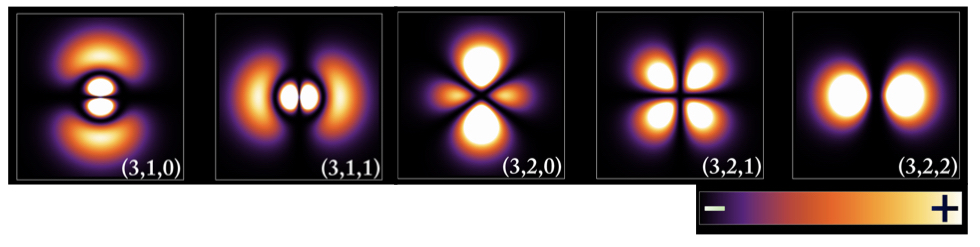
\includegraphics[width = 9cm]{Hubbard/Hydrogen.jpeg}
\caption[Hydrogen atomic wave functions.]{Probability density plots for different hydrogen orbital wave functions corresponding to quantum numbers $(n, l, m)$ for $n = 3$.
d-wave functions correspond to $l=2$.
We compare them with p-wave functions ($l=1$). The probability density is higher in a region near the nucleus, and its shape leads to a non-uniform distribution of electronic charge, as opposed to the case of the free electron gas. (adapted from \cite{hydrogen})}
\end{figure}

In a $d-$orbital, the electron charge density is concentrated near the nucleus.
In a solid, the electronic charge density should then also be concentrated near the nuclei, as long as the atomic description is useful, even if not completely correct\footnote{The electronic charge density is, of course, not actually defined in terms of a squared norm of the $d-$wave function for a narrow band. There is some broadening of the corresponding atomic energy level, and the wave function describing an electron is a Bloch wave function. Since the band is narrow, we assume that the atomic wave function description is still somewhat useful in a given range and we use it to provide a heuristic motivation for the non validity of the free electron assumption.}.
%It is much smaller between atoms so that electrons do seem to belong to individual atoms in some sense.
For a $d-$band, we assume this description to hold to some extent since the band is narrow.
The fact that we may speak with some meaning of an electron belonging to a particular atom motivates a description from which the atomic characteristics of the solid emerge, in spite of the fact that the bandwidth of a $d-$band is still appreciable.
The point is that electrons in $d-$bands are certainly not well described by a nearly free electron model nor by a tight biding model, which cannot possibly account for atomic-like behavior.

Experimentally, $d-$electrons of transition metals show hybrid behavior: sometimes they are accurately described by an ordinary band model, but there are occasions in which the atomic model is better.
For example, we see spin wave phenomena in ferromagnetic transition metals, and the susceptibilities of some of these metals depend strongly on temperature.
This is characteristic of an atomic (Heisenberg) model.
On the other hand, the $d-$electrons contribute significantly to the low temperature specific heat and sometimes the magnetic moments per atom of some transition metal ferromagnets are not integer multiples of the Bohr magneton.
This is characteristic of band theory\footnote{Think, for example, of a tight binding model. Electrons hop from atom to atom, and in general the spin of each atom depends on the particular electrons \say{belonging} to it at a given time. If we take an average of the total spin of each atom, we will in general not necessarily obtain an integer multiple of the Bohr magneton. If we simply had a collection of atoms, Hund's rule would apply, and each atom would have its spin aligned in a given direction. The average spin would then tend to be an integer multiple of the Bohr magneton.}.
Our theory of correlations should describe this balance between band-like and atomic-like behavior.

The atomic picture of a solid consists of an electron gas where ions are immersed.
The ions then interact in much the same way as they do in salts.
This extreme scenario is surely not even close to the true state of affairs since the number of $d-$electrons per atom is in general not an integer.
This motivates us to introduce a less restrictive model, which is not too far from the atomic model.
We shall assume that while $d-$electrons still have some band motion, they are strongly correlated with each other so that the solid retains some atomic-like behavior.
The correlations between electrons on different atoms are likely much weaker and we neglect them.

Let us now look at an example of the aforementioned circumstance.
Take a partially filled $d-$band of non-interacting electrons.
The spin of any given atom in the solid is just the total spin of all electrons on that atom.
It fluctuates both in magnitude and in direction, with a characteristic time that depends on how frequently $d-$electrons hop.
We can estimate the time interval between $d-$electron hopping events between atoms as a being of the order $\hbar / \Delta$, where $\Delta$ is the $d-$electron bandwidth.
The spin can thus be thought of as being associated to each individual (and constantly hopping) $d-$electron.

How do the electron interactions affect this picture?
We start by recalling Hund's rule: the nature of the  interactions between atoms leads to an alignment of the spins on each atom.
Since the atomic picture seems to prevail in our metal, we have reason to expect a similar effect to occur.
An atom with a total spin in some direction at a given time will tend to attract electrons with the spin on that direction and repel those with opposite spin.
This mechanism makes it unlikely for the spin of an atom to change much over time.
If the interactions between atoms are strong enough, the correlations become considerable and, making our statement  more precise, the total spin of an atom will persist for a time that is long compared with the $d-$electron hopping time.
Note that it is not the localization of the electrons that causes the spin state of the atom to persist.
The specific electrons belonging to a given atom change all the time as long as their spin is consistent with the total spin requirement imposed by Hund's rule.
For strong enough correlations, we may think of the spin as being associated to each atom, which opens up the possibility to describe the system using an atomic (Heisenberg) model, as we shall see later.

A theory of electron correlations in a narrow energy band should reduce to an atomic model in the appropriate limit, for example atoms that are so far apart on a lattice that they interact only very weakly.
Although we always keep in mind that we are focusing on $d-$electrons, we shall consider $s-$electrons in what follows for the sake of simplicity.
The important conclusions will not differ significantly.
We will use the "atomicity" of the electronic distribution to introduce an approximate representation of the electron interaction.
It turns out that this representation is mathematically much simpler to handle than the Coulomb interaction itself.

In short, our picture is the following: electrons hop rapidly from atom to atom in a band-like fashion, but their motion is correlated in such a way that atomic characteristics emerge.
The extent of atomic behavior depends, of course, on the strength of the interaction.

\subsection{Hubbard Hamiltonian}\label{subsec:hubbardHamiltonian}

Imagine a hypothetical partially filled narrow $s-$band with $n$ electrons per atom.
Suppose you have obtained Bloch wave functions $\psi_{\bm k}$ corresponding to energies $\varepsilon_{\bm k}$ by solving the Schr\"odinger equation for some spin-independent Hartree-Fock potential that accounts for the average interaction of the $s-$band electrons with electrons on other bands, and the interaction with the other $s-$electrons.
The electrons on the band evolve according to the Hamiltonian:
\begin{equation}\label{eq:startingHamiltonian}
\mathcal{H} = \sum_{\bm k \sigma} \bigg( \varepsilon_{\bm k} - \sum_{ \bm k'} \big( 2 V^{\bm k \bm k'}_{\bm k \bm k'} - V^{\bm k \bm k'}_{\bm k' \bm k} \big) \nu_{\bm k'} \bigg) c_{\bm k \sigma}^\dagger c_{\bm k \sigma} +  \frac{1}{2} \sum_{ \substack{\bm k_1 \bm k_2 \\ \bm k_1' \bm k_2'  \sigma_1 \sigma_2 } } V^{\bm k_1 \bm k_2}_{\bm k_1' \bm k_2'}
 c_{\bm k_1 \sigma_1}^\dagger c_{\bm k_2 \sigma_2}^\dagger c_{\bm k_2' \sigma_2} c_{\bm k_1' \sigma_1} ,
\end{equation}
where the $\bm k-$sums run over the first Brillouin zone.
The integrals are defined by
\begin{equation}\label{eq:integrals}
V^{\bm k_1 \bm k_2}_{\bm k_1' \bm k_2'} \equiv \left\langle \bm k_1 \bm k_2 \bigg| \frac{e^2}{r} \bigg| \bm k_1' \bm k_2' \right\rangle  =  e^2 \int \frac{\psi_{\bm k_1}^\star (\bm x) \psi_{\bm k_1'} (\bm x) \psi_{\bm k_2}^\star (\bm x') \psi_{\bm k_2'}(\bm x') }{| \bm x - \bm x' |} d\bm x d\bm x'
\end{equation}

The first term represents the band energies of the electrons minus their potential energy in the part of the Hartree-Fock field due to the electrons of the $s-$band itself.
The latter ensures that we do not overestimate the magnitude of the interactions between the electrons of the band: the Hartree-Fock field that specifies $\varepsilon_{\bm k}$ is computed taking into account these interactions, so if we didn't subtract it, we would count the energy of these interactions twice since they reappear in the last term, which  represents the interactions among all electrons in the system.
Furthermore, we assume that up and down spins are occupied equally, and $\nu_{\bm k}$ are the occupation numbers of the states of the band in the Hartree-Fock calculation. 
The term that we subtract in equation ($\ref{eq:startingHamiltonian}$) corresponds to the part of the interaction term which is already accounted for by the first diagonal \say{mean field} term.
Thus, it corresponds to the mean field expansion of the interaction term.
A generic way of writing the interaction term by gathering the $\bm k, \sigma$ indexes into a single index $\mu$ is $
V_{\text{int}} = \frac{1}{2} V^{\nu\mu}_{\nu'\mu'} c_\nu^\dagger c_\mu^\dagger c_{\mu'} c_{\nu'} ,
$
where the summation over repeated indexes is implied.
In appendix \ref{ap:hubbardObSol}, we obtain the form of $V_{\text{int}}$ in the Hartree-Fock approximation.

We may write the Bloch states $\psi_{\bm k}$ as a combination of Wannier functions localized at each atom.
\begin{equation}
\psi_{\bm k} (\bm x) = N^{-1/2} \sum_i e^{i \bm k \cdot \bm R_i} \phi (\bm x - \bm R_i), \,\, \text{where} \,\,\, \phi(\bm x) = N^{-1/2} \sum_{\bm k} \psi_{\bm k} (\bm x) , 
\end{equation}
and where $N$ is the number of atoms.
The sum runs over all atomic positions $\bm R_i$. 
Introducting the annihilation (creation) operators of an electron of spin $\sigma$ in the Wannier state $\phi (\bm x - \bm R_i)$ localized at site $i$, $c_{i\sigma}^{(\dagger)}$, we may write $
c_{\bm k \sigma}^{(\dagger)} = N^{-1/2} \sum_i e^{i \bm k \cdot \bm R_i} c_{i\sigma}^{(\dagger)}
$
, so that the Hamiltonian becomes 
\begin{equation}
\mathcal{H} = \sum_{\substack{ i j \\ \sigma} } K_{ij} c_{i \sigma}^\dagger c_{j \sigma} + \sum_{\substack{i j k l \\ \sigma \sigma'} } \bigg[  \frac{1}{2} V^{i j}_{k l}
 c_{i \sigma}^\dagger c_{j \sigma'}^\dagger c_{l \sigma'} c_{ k \sigma} - \bigg( 2 V^{i j}_{k l} - V^{i j} _{l k} \bigg) \nu_{j l} c_{i \sigma}^\dagger c_{ k \sigma} \bigg]  ,
\end{equation}
where
\begin{equation}\label{eq:hopping_matrix}
K_{ij} = N^{-1} \sum_{\bm k} \varepsilon_{\bm k} e^{i \bm k \cdot ( \bm R_i - \bm R_j )}, \, \text{and} \, \, \nu_{j l} = N^{-1} \sum_{\bm k} e^{i \bm k \cdot ( \bm R_j - \bm R_l) }
\end{equation}

Now comes the crucial approximation.
For a narrow energy band, the Wannier functions $\phi$ nearly coincide with atomic $s-$functions.
For small bandwidth, these $s-$functions form an atomic shell whose radius is small compared with the spacing between atoms, that is, the lattice constant.
Thus, the integral $U = \left\langle i i \big| e^2 / r \big| i i \right\rangle$ should turn out to be much larger than all other integrals.
This suggests the seemingly crude approximation of neglecting all other integrals.
However, this approximation is not so radical as it could seem at first sight since the other integrals are indeed much smaller than $U$.
In fact, for example, for $3d$ electrons of transition metals they are smaller by about two orders of magnitude \cite{hubbard_electron_1963}.
Keeping only the terms in $U$ in the interaction part, we obtain
\begin{equation}
\mathcal{H} = \sum_{i, j, \sigma} K_{ij} c_{i\sigma}^\dagger c_{j\sigma} + \frac{U}{2} \sum_{i\sigma} n_{i\sigma} n_{i, -\sigma} - U \sum_{i, \sigma} \nu_{i, i} n_{i, \sigma}
\end{equation}
where $n_{i\sigma} = c_{i\sigma}^\dagger c_{i\sigma}$.
Note that $\nu_{i, i} = N^{-1} \sum_{\bm k} \nu_{\bm k} = n/2$, where $n$ is the electron density, which means that the last term is constant and may be dropped.
Now, the hopping matrix $\bm K$ can, in principle, be found by inverse Fourier transforming the dispersion relation $\varepsilon_{\bm k}$ of the interaction-free system, that we can assume to be obtained experimentally or numerically.
From the tight binding view (with no $U$-term), we have a well defined crystal wavevectors that depend on the symmetry of the lattice, which may be written as Fourier transforms
$
\left| \bm k \right\rangle \equiv \frac{1}{N} \sum_{\bm r} e^{i\bm k \cdot \bm r} \left| \bm r \right\rangle , 
$
and, recalling the form of the hopping Hamiltonian (or the kinetic energy part in the Hubbard model):
$
\mathcal{H}_{K} = - \sum_{\bm r \bm r'} K (\bm r - \bm r') \left| \bm r' \right\rangle \left\langle \bm r \right| ,
$
 we can cast the dispersion relation as the (negative) Fourier transform of the hopping
\begin{equation}
- \mathcal{H}_{K} \left| \bm k \right\rangle = \frac{1}{\sqrt{N}} \sum_{\bm r \bm r'} K ( \bm r - \bm r' ) e^{i \bm k \cdot \bm r} \left| \bm r' \right \rangle = \frac{1}{\sqrt{N}} \bigg( \sum_{\bm R} K(\bm R) e^{i\bm k \cdot \bm R} \bigg)\bigg( \sum_{\bm r'} e^{i\bm k \cdot \bm r'} \left| \bm r' \right\rangle \bigg) = \varepsilon_{\bm k} \left| \bm k \right\rangle
\end{equation}

This gives us an interpretation of the $\bm K$ matrix: given the dispersion relation, and considering the solid to be well described by a tight binding model, we can easily obtain the matrix elements $K_{i j}$.

Let us now suppose that we have the simplest uniform nearest neighbor hopping model with Hubbard-type electron interactions.
Going back to equation (\ref{eq:hopping_matrix}), and recalling that the sum on $\bm k$ is restricted to the first Brillouin zone, we obtain the usual tight binding result: $K_{\left\langle i j \right\rangle} = - t \in \mathbbm{R}$ and $0$ otherwise (i.e. $\bm K$ is a very sparse matrix that is only non-zero for $i, j$ nearest neighbors).
Thus, the full Hamiltonian reads
\begin{equation}\label{eq:hubbard_hamiltonian}
\mathcal{H} = - t \sum_{\left\langle i, j \right\rangle, \sigma} \bigg(c_{i,\sigma}^\dagger c_{j,\sigma} + c_{j,\sigma}^\dagger c_{i,\sigma} \bigg) + U \sum_{i} n_{i,\uparrow} n_{i\downarrow} -\mu \sum_i \bigg( n_{i,\uparrow} + n_{i,\downarrow} \bigg) ,
\end{equation}
where, for generality, we included the chemical potential, thus taking the \acl{GCE}.

\subsection{Particle-hole symmetry}

In this section we examine a particularly relevant and unique symmetry of the Hubbard model.
The main idea is that, at half filling, the Hubbard Hamiltonian is invariant under a transformation which turns particles into holes and vice-versa.
\ac{PHS} allows us to relate the properties of the Hubbard Hamiltonian at different values of the parameters.
Moreover, it allows us to devise a mapping between the attractive ($U < 0$) and the repulsive ($U > 0$) models.
We will see later that this mapping is important in QMC simulations \cite{alavi_quantum_2016}.
We start our discussion with the concept of a bipartite lattice.
A lattice is said to be bipartite if it can be divided into two sublattices $\mathcal{A}$ and $\mathcal{B}$, such that the set of neighbors of a site in sublattice $\mathcal{A}$ belongs to sublattice $\mathcal{B}$.
For example, the square and honeycomb lattices are bipartite, whereas the triangular lattice is not.
In a bipartite lattice, antiferromagnetic (\acs{AF}) order is favored.
In contrast, \acs{AF} order is frustrated on the triangular and other non bipartite lattices.
%\begin{figure}[H]\label{fig:bipartite}
%\centering
%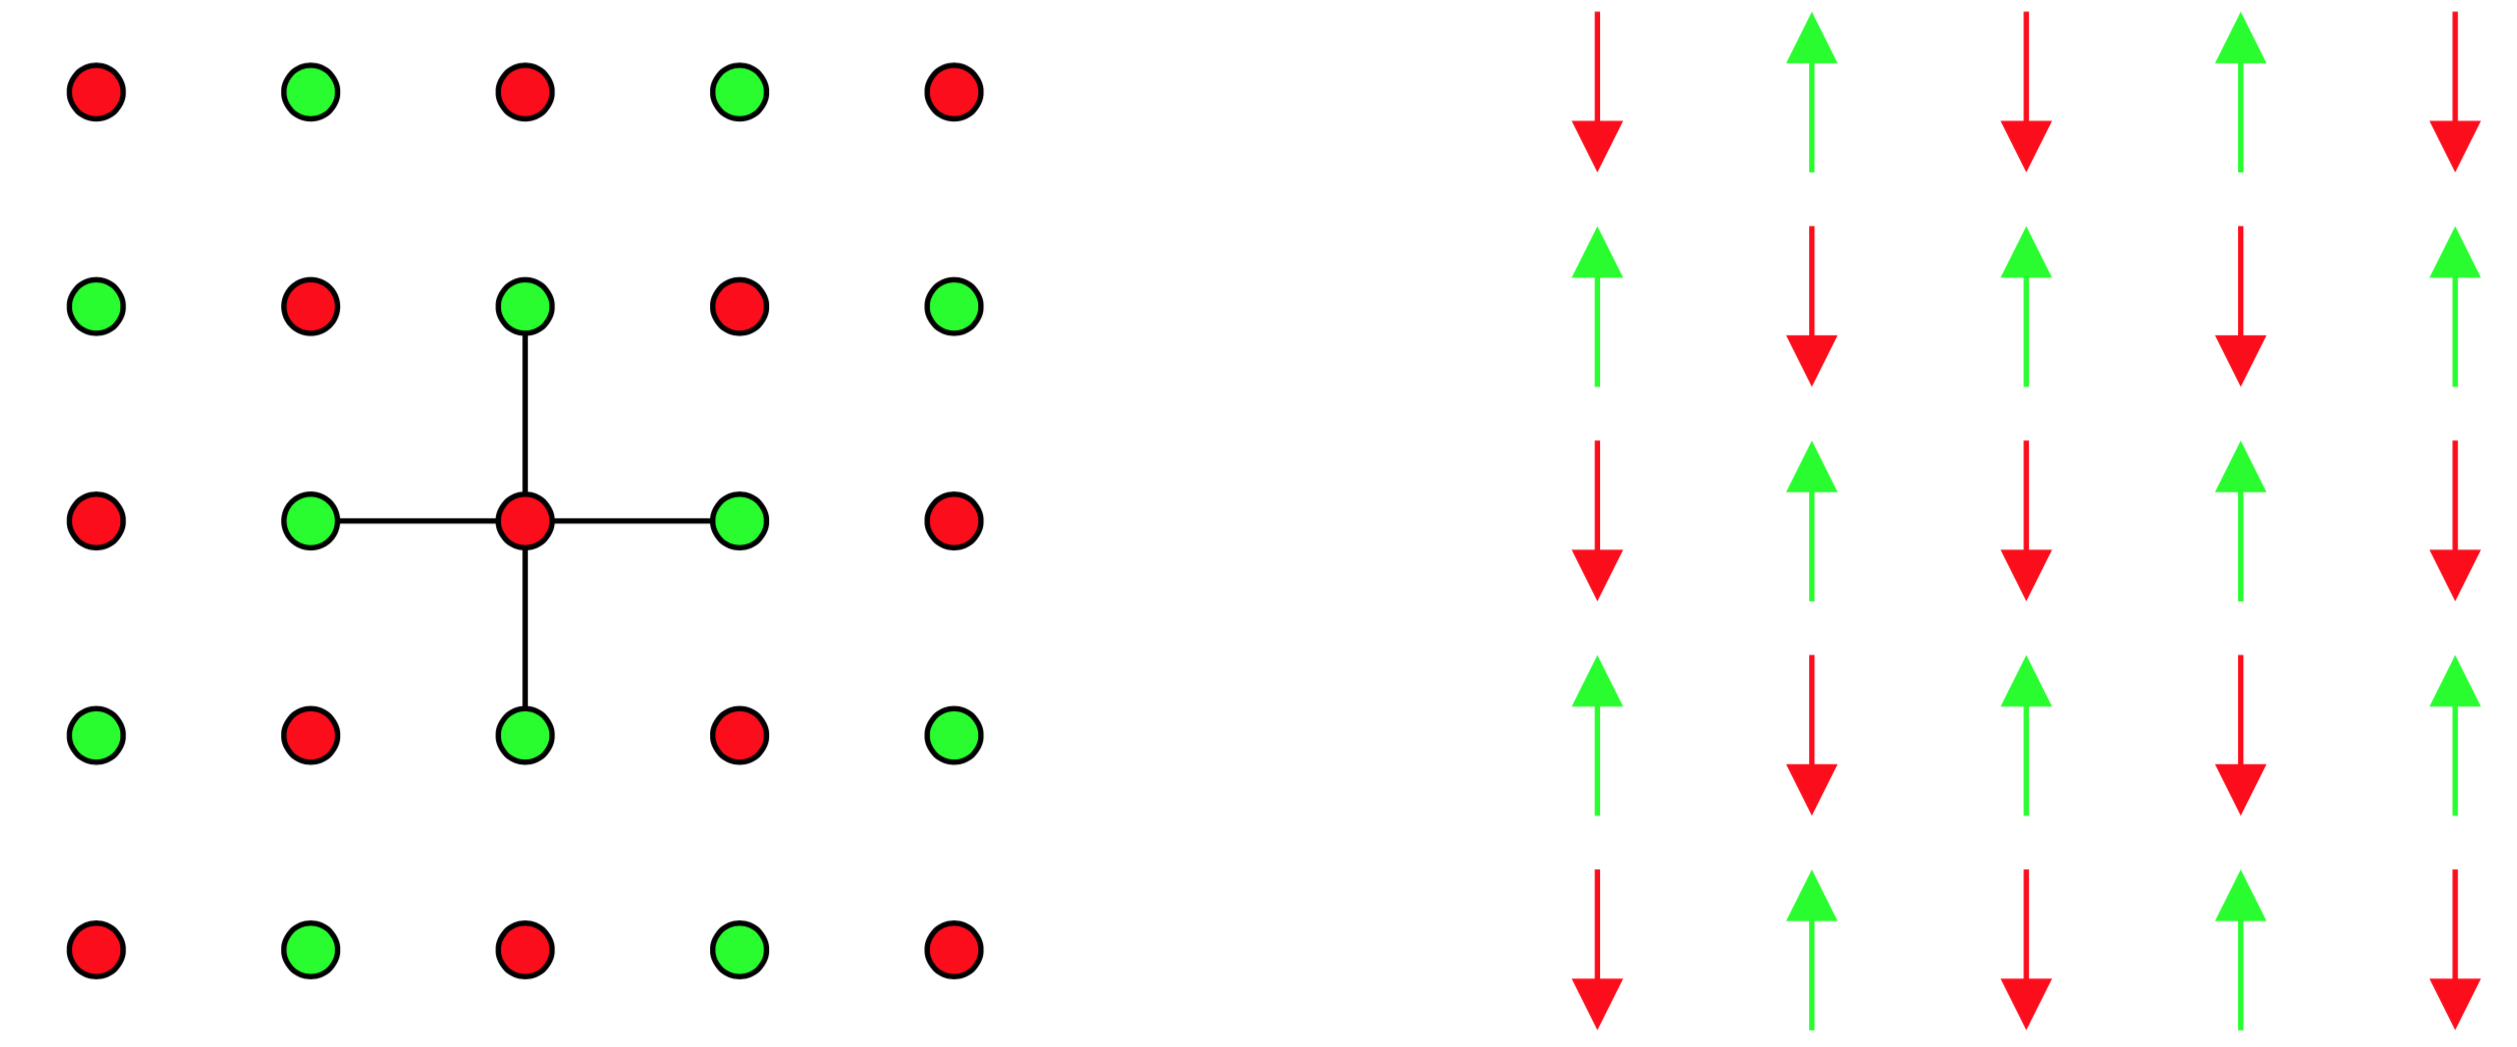
\includegraphics[width = 5.2cm]{Hubbard/bipartite}
%\caption[Bipartite lattices and antiferromagnetic order.]{On the left, we see that the square lattice is bipartite.
%The neighbors of a particular site in the red sublattice all belong to the green sublattice.
%The picture on the right is meant to give some intuition on why the bipartite lattice favors \ac{AF} order.
%We represent a configuration where fermions of a given spin have as their neighbors only fermions of opposite spin, which would be favored by Heisenberg exchange (taken from \cite{alavi_quantum_2016}). }
%\end{figure}

Introducing a \ac{PHT},
\begin{equation}\label{eq:PHT}
d_{ i, \sigma}^\dagger = (-1)^i c_{i, \sigma} ,
\end{equation}
we exchange the role of annihilation and creation operators.
In fact, particles become holes and vice-versa: $d_{ i, \sigma}^\dagger d_{ i, \sigma} = 1 - c_{ i, \sigma}^\dagger c_{ i, \sigma} $, and the occupations $n = 0, 1$ are interchanged.
Consider a bipartite lattice.
Since in that case the factor $(-1)^i$ takes on $-1$ on one sublattice and $1$ on the other, the kinetic part of the Hamiltonian is invariant under a \ac{PHT}: $
c_{i, \sigma}^\dagger c_{j, \sigma} + c_{j, \sigma}^\dagger c_{i, \sigma} \mapsto (-1)^{i+j} ( d_{i, \sigma} d_{j, \sigma}^\dagger + d_{j, \sigma} d_{i, \sigma}^\dagger ) = d_{j, \sigma}^\dagger d_{i, \sigma} + d_{i, \sigma}^\dagger d_{j, \sigma}
$.

The \ac{PHS} form of the kinetic term can be incorporated into the interaction term by a shift in the chemical potential and by adding a constant to the Hamiltonian.
First, note that the interaction term $
U \big( n_{i,\uparrow} - \frac{1}{2} \big) \big( n_{i,\downarrow} - \frac{1}{2} \big)
$
is unchanged under a \ac{PHT}.
Expanding it, we get $U n_{i,\uparrow} n_{i,\downarrow} - \frac{U}{2} (n_{i,\uparrow} + n_{i,\downarrow}) + \frac{U}{4}$, which indeed differs from the original interaction term by a shift in the chemical potential ($\mu \rightarrow \mu + U / 2$) plus a constant.
Thus, the particle-hole symmetric Hamiltonian is equivalent to the original one.
\begin{equation}
\mathcal{H} = -t \sum_{\left\langle i, j \right \rangle, \sigma} \bigg( c_{i,\sigma}^\dagger c_{j,\sigma} + c_{i,\sigma}^\dagger c_{j,\sigma} \bigg) + U \sum_{i} \bigg( n_{i,\uparrow} - \frac{1}{2} \bigg) \bigg( n_{i,\downarrow} - \frac{1}{2} \bigg) -\mu \sum_i \bigg( n_{i,\uparrow} + n_{i,\downarrow} \bigg)
\end{equation}

Under a \ac{PHT}, the density, $\rho = \left\langle n_\uparrow + n_\downarrow \right\rangle$, transforms as $\rho \mapsto 2 - \rho$.
The Hamiltonian changes only in the chemical potential term: $\mu \mapsto -\mu$.
Thus, we have that $\rho (\mu) = 2 - \rho (-\mu)$, and at $\mu = 0$, we have half filling: $\rho = 1$.
This reasoning is valid for any $\beta$, $t$, or $U$, which implies that the phase diagram of the Hubbard model must be symmetric about half filling.
Suppose you added next nearest neighbor (NNN) hoppings $t'$\footnote{On the square lattice, this corresponds to connecting sites across the diagonal of each square.}.
Then, \ac{PHS} would be broken, and the phase diagram would no longer be symmetric about $\mu = 0$.
Indeed, a modified version of the Hubbard model with NNN hoppings is often used to model cuprate superconductors, and this lack of symmetry is consistent with the fact that hole- and electron-doped cuprates have different properties. 
\ac{PHS} is also broken for the triangular lattice with non uniform hoppings we shall consider later when modelling \acp{TMD}.
\section{Mott insulators}\label{sec:mott}

Band theory was found to be flawed soon after it was introduced.
The picture it proposes is simple and generally works pretty well.
It is based on considering the electrons to be independently moving under the constant background potential created by the ions.
The solutions of the Schr\"odinger for free electrons in a periodic potential $U(\bm r)$, such that $U(\bm r) = U(\bm r + \bm R)$,

\begin{equation}\label{eq:schrodinger}
\bigg[ -\frac{1}{2m} \nabla^2 + U(\bm r) \bigg] \psi (\bm r) = \varepsilon \psi (\bm r)
\end{equation}
are given by Bloch's theorem: $\psi_{\bm k} (\bm r) = e^{i\bm k \cdot \bm r} u_{\bm k} (\bm r)$.
Note that we made $\hbar = 1$.
Replacing this wave function in equation (\ref{eq:schrodinger}), we obtain a differential equation for $u_{\bm k} (\bm r)$, which has in general an infinite number of solutions.
We label them with an index $n$, which we call the band index.
To each solution there corresponds a function $\varepsilon_{n\bm k}$.
The set of these functions is known as the band structure.
Since electrons are taken to be independent in band theory, the N-electron eigenstates are obtained by placing an electron in each quantum state.
Each state is labelled by its energy $\varepsilon_{n\bm k \sigma}$.
Since our model Hamiltonian does not couple spins (via an electron interaction, for example) and assuming there is no external magnetic field and that the system has an inversion center, we have $\varepsilon_{n\bm k \uparrow} = \varepsilon_{n\bm k \downarrow}$.
In general there might be energies for which there is no corresponding $\varepsilon_{n\bm k \sigma}$.
These form intervals called forbidden bands\footnote{We disregard surface states that may have energies that fall in the forbidden bands of band theory.}.
Thus, the ground state of our model may be obtained by filling the energy levels starting from the lowest energy state.
Two cases are particularly relevant:
\begin{itemize}
\item Every band is either fully occupied or empty.
The first excited state differs from the ground state by $\Delta$, the separation between the last fully occupied band and the first empty band.
It is then impossible to induce the motion of the electrons by applying an arbitrarily small voltage.
This is what it means to be an \emph{insulator}.
Since there $2N$ states per band, this is not possible unless the number of electrons per unit cell is an even integer.
\item One or more of the bands are partially filled.
The energy of occupied state of higher energy is named the Fermi energy $\varepsilon_F$.
In this case, the separation between the ground state and the first excited state tends to $0$ in the thermodynamic limit, $N \rightarrow \infty$.
The system may then respond to infinitesimal excitations, which is the definition of a metal.
\end{itemize}

Band theory made it possible to predict whether a solid would be a metal or an insulator.
However, its success rests crucially on the independent electron approximation.
Thus, it is not surprising that for compounds with strongly correlated electrons the theory might fail \cite{mila_physique_2007}.
The Coulomb interaction is in general non negligible, and the effects it leads to are not captured by a mean field approach.
One must resort to many-body theory.
An example of a many-body effect that band theory doesn't capture is  superconductivity.
However, this does not deem band theory useless.
In fact, the superconducting phase arises due to an instability of a state that is itself well described by band theory \cite{gennes_superconductivity_1999}.
A far greater failure of band theory is that predicts certain compounds with an odd number of electrons per unit cell, such as \chem{NiO} and \chem{La_2 Cu O_4},  to be metals, while in fact  they turn out to be (Mott) insulators.
Mott devised a simple argument to justify this failure.
It is based on considering the elementary electronic excitations of a solid composed by hydrogen atoms as a function of the distance between atoms.

Consider a hypothetical solid consisting of a square lattice with hydrogen atoms on its points.
Each unit cell has one hydrogen atom, and consequently one electron.
Band theory would predict such a solid to be a metal.
However, if the lattice parameter $a$ is large enough, the solid cannot remain a metal.
There must be some value of the lattice parameter $a = a_c$ for which the system becomes an insulator.
When current flows through a sample of this solid, electrons hop consecutively, reaching positions that can be quite far on the lattice.
For a metal, this process occurs even when exciting the system with an infinitesimal amount of energy.
How much energy do we need to provide for this process to occur?

\begin{figure}[ht!]\label{hubbardOneHoleOneDoublyOc}
\centering
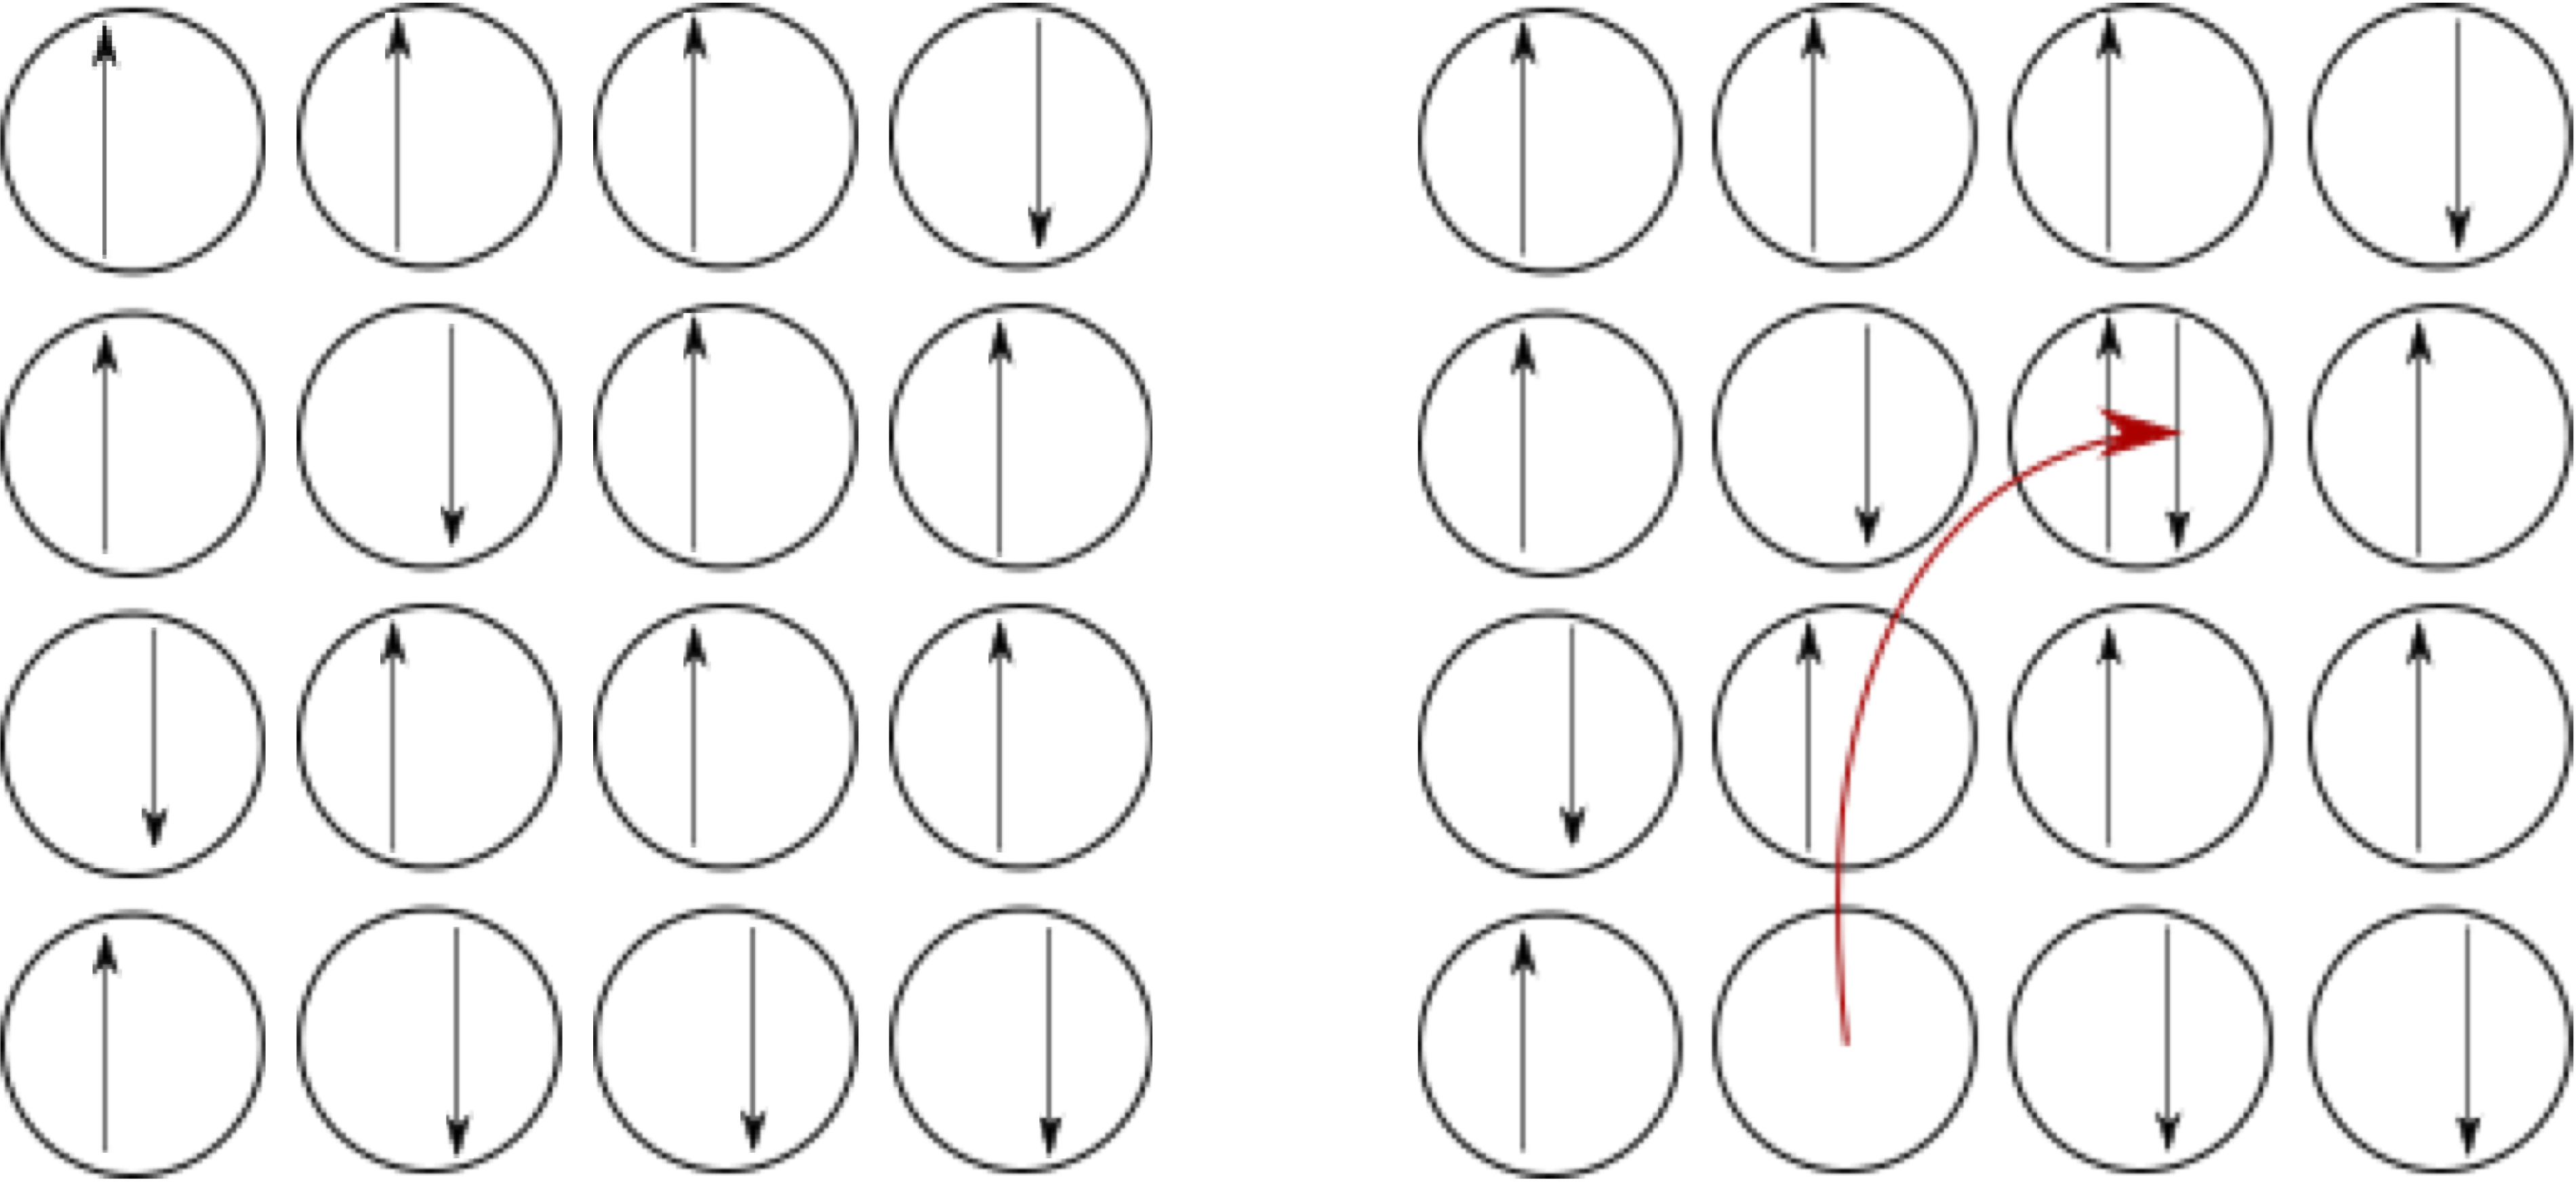
\includegraphics[width = 9cm]{Hubbard/hubbardOneHoleOneDoublyOcV2.png}
\caption[Configuration of the Hubbard model on the square lattice with a hole and a doubly occupied site.]{On the right, a configuration of hydrogen atoms on a square lattice with a hole and a doubly occupied site obtained by delocalization of the spin down electron on the left.}
\end{figure}

If $a$ is large, we have essentially one electron per site at the start.
When an electron is displaced, we end up with a hole and a doubly occupied site.
The potential energy of such a state is

\begin{equation}
E_{H^-} + E_{H^+} - 2 E_H 
\end{equation}

Due to the Coulomb repulsion between the two electrons in $H^-$, this quantity is strictly positive.
Call it $U > 0$.
On the other hand, the system also has kinetic energy: both the hole and the doubly occupied site can delocalize.
Let $W$ be the bandwidth corresponding to the delocalization of an electron on the lattice.
Both the hole and the doubly occupied will stay at the bottom of the band and gain an energy $W/2$ (assuming that this delocalization is of the same order of magnitude).
The dominant transfer integral $-t$ is between nearest neighbors.
The dispersion relation then reads

\begin{equation}
\varepsilon_{\bm k} = -2 t ( \cos k_x + \cos k_y ) 
\end{equation}

The bandwidth is then $W = 8 t$.
The energy of a configuration with a hole and a doubly occupied site is

\begin{equation}
\Delta_c = U - W ,
\end{equation}
where $U$ is practically independent of the lattice parameter $a$.
The bandwidth $W$, however, depends strongly on $a$.
When $a \gg a_0$, where $a_0$ is the Bohr radius, the transfer integral is exponentially small, because only the exponential tails of the wave functions are relevant.
In this limit, $\Delta_c \approx U$ is a large, positive number, and the system is an insulator.
This type of insulator is called a Mott insulator, and $\Delta_c$ is called the charge gap.
As $a$ decreases, $t$ increases, and there must be a critical value $a_c \sim a_0$, for which $U = W$.
Below this value, the computation of $\Delta_c$ is not valid anymore because the gap cannot be negative.
Thus, there must be a metal-insulator transition.
It is possible to see this transition if we apply enough pressure to a Mott insulator so as to decrease $a$ and increase $t$.
A transition of this type was first seen in the 1970's for $V_2 O_3$\footnote{Of course, the transition is not so easy to describe. We should consider the Hubbard model!
However, this simple argument provides an intuitive picture.}.
There is a fundamental difference between a band insulator and a Mott insulator.
While we must pay an energy $\Delta_c$ to make a charge excitation, there is no cost for making a spin excitation: we can flip the spin of an electron without creating a doubly occupied site.
The fluctuations of both charge and spin due to the electron interactions may then lead to magnetic behavior characteristic of correlated  systems.
\section{Exact solutions for simple cases}\label{sec:exactSolutions}

In \ac{PHS} form, the Hubbard Hamiltonian may then be written as a sum of kinetic, chemical and potential energy terms, respectively:

\begin{equation}\label{eq:hubbard}
\mathcal{H} = \mathcal{H}_K + \mathcal{H}_\mu + \mathcal{H}_V ,
\end{equation}
defined as

\begin{equation}\label{eq:def_energies}
\mathcal{H}_K = -t \sum_{\left\langle i, j \right \rangle, \sigma} \bigg( c_{i,\sigma} c_{j,\sigma}^\dagger + c_{j,\sigma}^\dagger c_{i,\sigma} \bigg) , \,\,\,
\mathcal{H}_\mu = -\mu \sum_i \bigg( n_{i,\uparrow} + n_{i,\downarrow} \bigg) , \,\,\,
\mathcal{H}_V = U \sum_{i} \bigg( n_{i,\uparrow} - \frac{1}{2} \bigg) \bigg( n_{i,\downarrow} - \frac{1}{2} \bigg) ,
\end{equation}
where:

\begin{itemize}
\item $i$ and $j$ label sites on the lattice.
\item $c_{i,\sigma}^{(\dagger)}$ is an operator that annihilates (creates) an electron with spin $\sigma$ on site $i$.
\item $n_{i,\sigma}$ is the number operator counting the number of electrons of spin $\sigma$ on site $i$ (either 0 or 1).
\item $t$ is the hopping parameter related to the kinetic energy of the electrons.
It is determined by the overlap of the atomic wave functions on neighboring sites $\left\langle i, j \right\rangle$.
\item $U$ is the on-site Coulomb repulsion between electrons.
Whenever a site $i$ has two electrons, there is a local repulsion between them corresponding to an energy cost $U n_{i \uparrow} n_{i \downarrow}$ (up to an additive constant).
\item $\mu$ is the chemical potential controlling the electron number (or density).
\end{itemize}

A given physical observable of interest $\mathcal{O}$, such as the spin-spin correlation, or the magnetic susceptibility may be computed formally by

\begin{equation}
\left\langle \mathcal{O} \right\rangle = \text{Tr} ( \mathcal{O} \mathcal{P} )
\end{equation}
where

\begin{equation}\label{eq:projection}
\mathcal{P} \equiv \frac{1}{Z} e^{-\beta \mathcal{H} } , \text{ with } Z = \text{Tr} ( e^{-\beta \mathcal{H} } )
\end{equation}

The trace is taken over the Hilbert space corresponding to all possible configurations of the lattice occupation.
Defining an orthonormal basis of this Hilbert space $\{ | \psi_\alpha \rangle | \alpha = 1, ... D \} $, where $D$ is the dimension of the Hilbert space, the partition function reads

\begin{equation}\label{eq:z_asEigen}
\Tr ( e^{-\beta \mathcal{H} } )= \sum_\alpha \left\langle \psi_\alpha | e^{-\beta \mathcal{H} } | \psi_\alpha \right\rangle
\end{equation}

There are four possible states at each site in the Hubbard model: $\left| \,\, \right\rangle$, $\left|\uparrow \right\rangle$, $\left|\downarrow\right \rangle$, $\left|\uparrow \downarrow \right\rangle $, corresponding, respectively, to no electron, a spin up or spin down electron, and two electrons of opposite spin occupying the site.
The potential energy operator acts as follows

\begin{equation}
U (n_{i\uparrow} - \frac{1}{2} ) ( n_{i\downarrow} - \frac{1}{2} ) 
\begin{cases}
\left| \,\, \right\rangle = \frac{U}{4} \left| \,\, \right\rangle \\
\left|\uparrow \right\rangle = -\frac{U}{4} \left|\uparrow \right\rangle \\
\left|\downarrow\right \rangle = -\frac{U}{4} \left|\downarrow\right \rangle \\
\left|\uparrow \downarrow \right\rangle = \frac{U}{4} \left|\uparrow \downarrow \right\rangle \\
\end{cases}
\end{equation}

Singly occupied states ($\left|\uparrow \right\rangle$, $\left|\downarrow\right \rangle$) have lower energy and are thus more likely to occur.
They correspond to nonzero magnetization $m = n_{\uparrow} - n_{\downarrow}$, which is favored by the Hubbard interaction $U$.
A relevant question is whether or not the spins order in space when $t \neq 0$ and to what extent.

Let us now establish our notations for second quantized operators to introduce a different representation of electronic states on the lattice.
The fermionic annihilation and creation operators anticommute:
$\{ c_{j\sigma} , c_{l \sigma'}^\dagger \} = \delta_{jl} \delta_{\sigma\sigma'}$.
The $c$-operator algebra is further defined by the vanishing of all other anticommutators:$
\{ c_{j\sigma}^{(\dagger)} , c_{l \sigma'}^{(\dagger)} \} = 0$.
Note that taking $l = j$ and $\sigma = \sigma'$ in this equation for the $c^\dagger$-operators, we recover Pauli's exclusion principle since $(c_{j\sigma}^\dagger)^2 = 0$.
If we omit the site $i$ and spin $\sigma$ indices, a convenient way of specifying states on the lattice is

\begin{equation}
\left| 0 \right\rangle : \text{unoccupied state - no electron} \,\,\,\, \left| 1 \right\rangle : \text{occupied state - one electron}
\end{equation}
so that a generic state may be written as a product of the states above $\otimes_{i=1}^{N} \otimes_{\sigma = \pm 1/2} \left| n \right\rangle_{i, \sigma}$ at each site for each spin state, where $n= 0, 1$.
For example, one such state is

\begin{equation}
\left| 0 \right\rangle_{1, \uparrow} \left| 1 \right\rangle_{1, \downarrow} \left| 1 \right\rangle_{2, \uparrow} \left| 1 \right\rangle_{2, \downarrow} \left| 0 \right\rangle_{3, \uparrow} \left| 0 \right\rangle_{3, \downarrow} ... \left| 1 \right\rangle_{N, \uparrow} \left| 0 \right\rangle_{N, \downarrow}  ,
\end{equation}
where $N$ is the number of sites on the lattice. Site $1$ has a single spin-down electron, while site $2$ is doubly occupied, site $3$ is unoccupied, and so on, until we reach site $N$, which has a single spin-up electron.

The creation and annihilation operators act as follows

\begin{equation}
c \left| 0 \right\rangle = 0 \quad c^\dagger \left| 0 \right\rangle = \left| 1 \right\rangle \quad c \left| 1 \right\rangle = \left| 0 \right\rangle \quad c^\dagger \left| 1 \right\rangle = 0
\end{equation}

Thus, the eigenstates of the number operator are $\left| 0 \right\rangle, \left| 1 \right\rangle$: $
n \left| 0 \right\rangle = 0 , \quad n \left| 1 \right\rangle = \left| 1 \right\rangle
$.

Moreover, the operator $c_i^\dagger c_{i+1}^\dagger$, corresponding to the hopping from site $i+1$ to $i$, i.e. to the kinetic energy of the electrons on neighboring sites, acts as follows (ignoring spin):

\begin{equation}
c_i^\dagger c_{i+1}^\dagger \begin{cases}
\left|0 0 \right\rangle = 0 \\
\left|1 0 \right\rangle =  0 \\
\left|0 1 \right\rangle =  \left| 1 0 \right\rangle \\
\left|1 1 \right\rangle =  c_i^\dagger \left| 1 0  \right\rangle = 0 \\
\end{cases}
\end{equation}

The operator annihilates the particle at $i+1$ and creates it back at $i$, i.e. the electron hops from $i+1$ to $i$.

\subsection{The purely atomic ( $\frac{t}{U} = 0$ ), single site limit}
\label{subsec:atomic}

When $t = 0$, the site index may be omitted since the Hamiltonian is a sum of operators solely at site $i$.
Hence, we have $[ \mathcal{H}, n_{i,\sigma} ] = 0 \,\, \forall i = 1, 2,..., N $, and the eigenstates of $\mathcal{H}$ are also eigenstates of all number operators at the different sites in the lattice.
Thus, in the single site limit, we obtain

\begin{equation}
\mathcal{H} = U \bigg(n_\uparrow - \frac{1}{2} \bigg) \bigg(n_\downarrow - \frac{1}{2} \bigg) - \mu \bigg( n_\uparrow + n_\downarrow \bigg)
\end{equation}
which acts as follows (using the eigenstates of $n_\sigma$)

\begin{equation}
\mathcal{H} \begin{cases}
\left| \,\, \right\rangle = \frac{U}{4} \left| \,\, \right\rangle \\
\left| \uparrow \right\rangle = \bigg( \frac{U}{4} - (\mu + \frac{U}{2} ) \bigg) \left| \uparrow \right\rangle \\
\left| \downarrow \right\rangle = \bigg( \frac{U}{4} - (\mu + \frac{U}{2} ) \bigg) \left| \downarrow \right\rangle \\
\left| \uparrow \downarrow \right\rangle = \bigg( \frac{U}{4} - 2 \mu \bigg) \left| \uparrow \downarrow \right\rangle
\end{cases}
\end{equation}

Thus, the Hamiltonian is diagonal in the basis $\{\left| \psi_\alpha \right\rangle \} = \left| \,\, \right\rangle, \left|\uparrow \right\rangle, \left|\downarrow\right \rangle, \left|\uparrow \downarrow \right\rangle $:

\begin{equation}
\mathcal{H} \leadsto \bm H = \text{diag}\bigg(\frac{U}{4}, \frac{U}{4} - (\mu + \frac{U}{2} ), \frac{U}{4} - (\mu + \frac{U}{2} ), \frac{U}{4} - 2 \mu \bigg) ,
\end{equation}
which means that $e^{-\beta \mathcal{H} }$ is also diagonal:

\begin{equation}
e^{-\beta \mathcal{H} } \leadsto e^{-\beta U / 4}  \text{diag}\bigg(1,  e^{\beta(\mu + \frac{U}{2})}, e^{\beta(\mu + \frac{U}{2})},  e^{2\beta \mu} \bigg)
\end{equation}
and this is one of the rare situations in which it is possible to explicitly write down a closed form for the partition function.

\begin{equation}\label{eq:singleSitePartition}
Z = \text{Tr} [ e^{-\beta\mathcal{H} } ] = \sum_\alpha \left\langle \psi_\alpha \left|e^{-\beta \mathcal{H} } \right| \psi_\alpha \right\rangle = e^{-\beta U / 4} \bigg(1 + 2 e^{\beta(\mu + \frac{U}{2})} + e^{2 \beta \mu} \bigg)
\end{equation}

Moreover, some of the observables that were mentioned before are explicitly computable.
This is because due to the diagonal form of $\mathcal{H}$, the expressions defining these observables greatly simplify.

\begin{equation}
\begin{split}
\mathcal{H} e^{-\beta\mathcal{H} } &\leadsto e^{-\beta U / 4}  \text{diag}\bigg(\frac{U}{4}, (-\mu - \frac{U}{4})  e^{\beta(\mu + \frac{U}{2})} (-\mu - \frac{U}{4}) e^{\beta(\mu + \frac{U}{2})}, (\frac{U}{4} - 2\mu ) e^{2\beta \mu} \bigg) \\
n_{\uparrow} e^{-\beta\mathcal{H} } &\leadsto e^{-\beta U / 4}  \text{diag}\bigg(0, e^{\beta(\mu + \frac{U}{2})}, 0,  e^{2\beta \mu} \bigg) \\
n_{\downarrow} e^{-\beta\mathcal{H} } &\leadsto e^{-\beta U / 4}  \text{diag}\bigg(0, 0, e^{\beta(\mu + \frac{U}{2})},   e^{2\beta \mu} \bigg) \\
n_{\uparrow} n_{\downarrow} e^{-\beta\mathcal{H} } &\leadsto e^{-\beta U / 4}  \text{diag}\bigg(0, 0, 0,   e^{2\beta \mu} \bigg) \\
\end{split}
\end{equation}

From these we can compute some traces which we shall find useful to obtain averages of various observables.

\begin{equation}
\begin{split}
&\Tr \bigg[ \mathcal{H} e^{-\beta\mathcal{H} } \bigg] = e^{-\beta U / 4} \bigg(\frac{U}{4} + 2 (-\mu - \frac{U}{4})  e^{\beta(\mu + \frac{U}{2})} + (\frac{U}{4} - 2\mu ) e^{2\beta \mu} \bigg) \\
&\Tr \bigg[ (n_\uparrow + n_\downarrow ) e^{-\beta\mathcal{H} } \bigg] = e^{-\beta U / 4} \bigg(2 (-\mu - \frac{U}{4})  e^{\beta(\mu + \frac{U}{2})} + (\frac{U}{4} - 2\mu ) e^{2\beta \mu} \bigg) \\
&\Tr \bigg[ n_\uparrow n_\downarrow \bigg] = e^{-\beta U/4} e^{2\beta\mu}
\end{split}
\end{equation}

The bottom line is that we are able to obtain \emph{exact} expressions for

\begin{enumerate}
\item the one-site density $\rho = \left\langle n_\uparrow \right\rangle + \left\langle n_\downarrow \right\rangle$, measuring the average occupation of each site.
\begin{equation}
\rho = \frac{\text{Tr} \big[ (n_\uparrow + n_\downarrow ) e^{-\beta\mathcal{H}} \big]}{Z} = \frac{2 e^{\beta(\frac{U}{2} + \mu)} + 2 e^{2\beta\mu}}{1 + 2 e^{\beta(\mu + \frac{U}{2})} + e^{2 \beta \mu}}
\end{equation}

Note that when there is no chemical potential $\mu = 0$, we have $\rho = 1$ for any $U$, or $\beta$.
This corresponds to half filling: the density of electrons is half its maximum possible value.

In figure (\ref{fig:rhoVsMu}), we plot $\rho(\mu)$ for varying temperature, and fixed on-site interaction.
It allows us to get some insight into the Mott insulating gap.
At $T = 0.25$, the curve owes its step-like shape to the small thermal fluctuations.
As $T$ increases, the curve starts losing this tendency, and by $T = 2.0$, it is no longer possible to identify it.
This is a consequence of the now larger thermal fluctuations that are present at higher temperature.

We denote the flat region between $\mu = - U / 2 $ and $\mu =  U / 2 $  \say{Mott Plateau}.
As the chemical potential is increased, the density remains small until a threshold is exceeded at $\mu = - \frac{U}{2}$. 
Then, it rises very rapidly to $\rho = 1$ (half filling), and again stays almost constant.
It is not until $\mu$ jumps by $U$ that we fill the site ($\rho = 2$).
This Mott insulating gap appears because the presence of a fermion in the site blocks the addition of a second due to the on-site interaction.
One needs a sufficiently large chemical potential to overcome this effect.
As we shall see, this feature of the model remains present as the number of sites increases.
Note that in the Mott gap, the compressibility vanishes: $\kappa = \frac{\partial \rho}{\partial \mu} = 0$.

Just as thermal fluctuations can destroy the sharp jumps corresponding to the gap, so can quantum fluctuations.
The hopping term in the Hamiltonian introduces such fluctuations, leading to an effect similar to that of figure (\ref{fig:rhoVsMu}).

\begin{figure}[H]
	\centering
\hspace{12mm}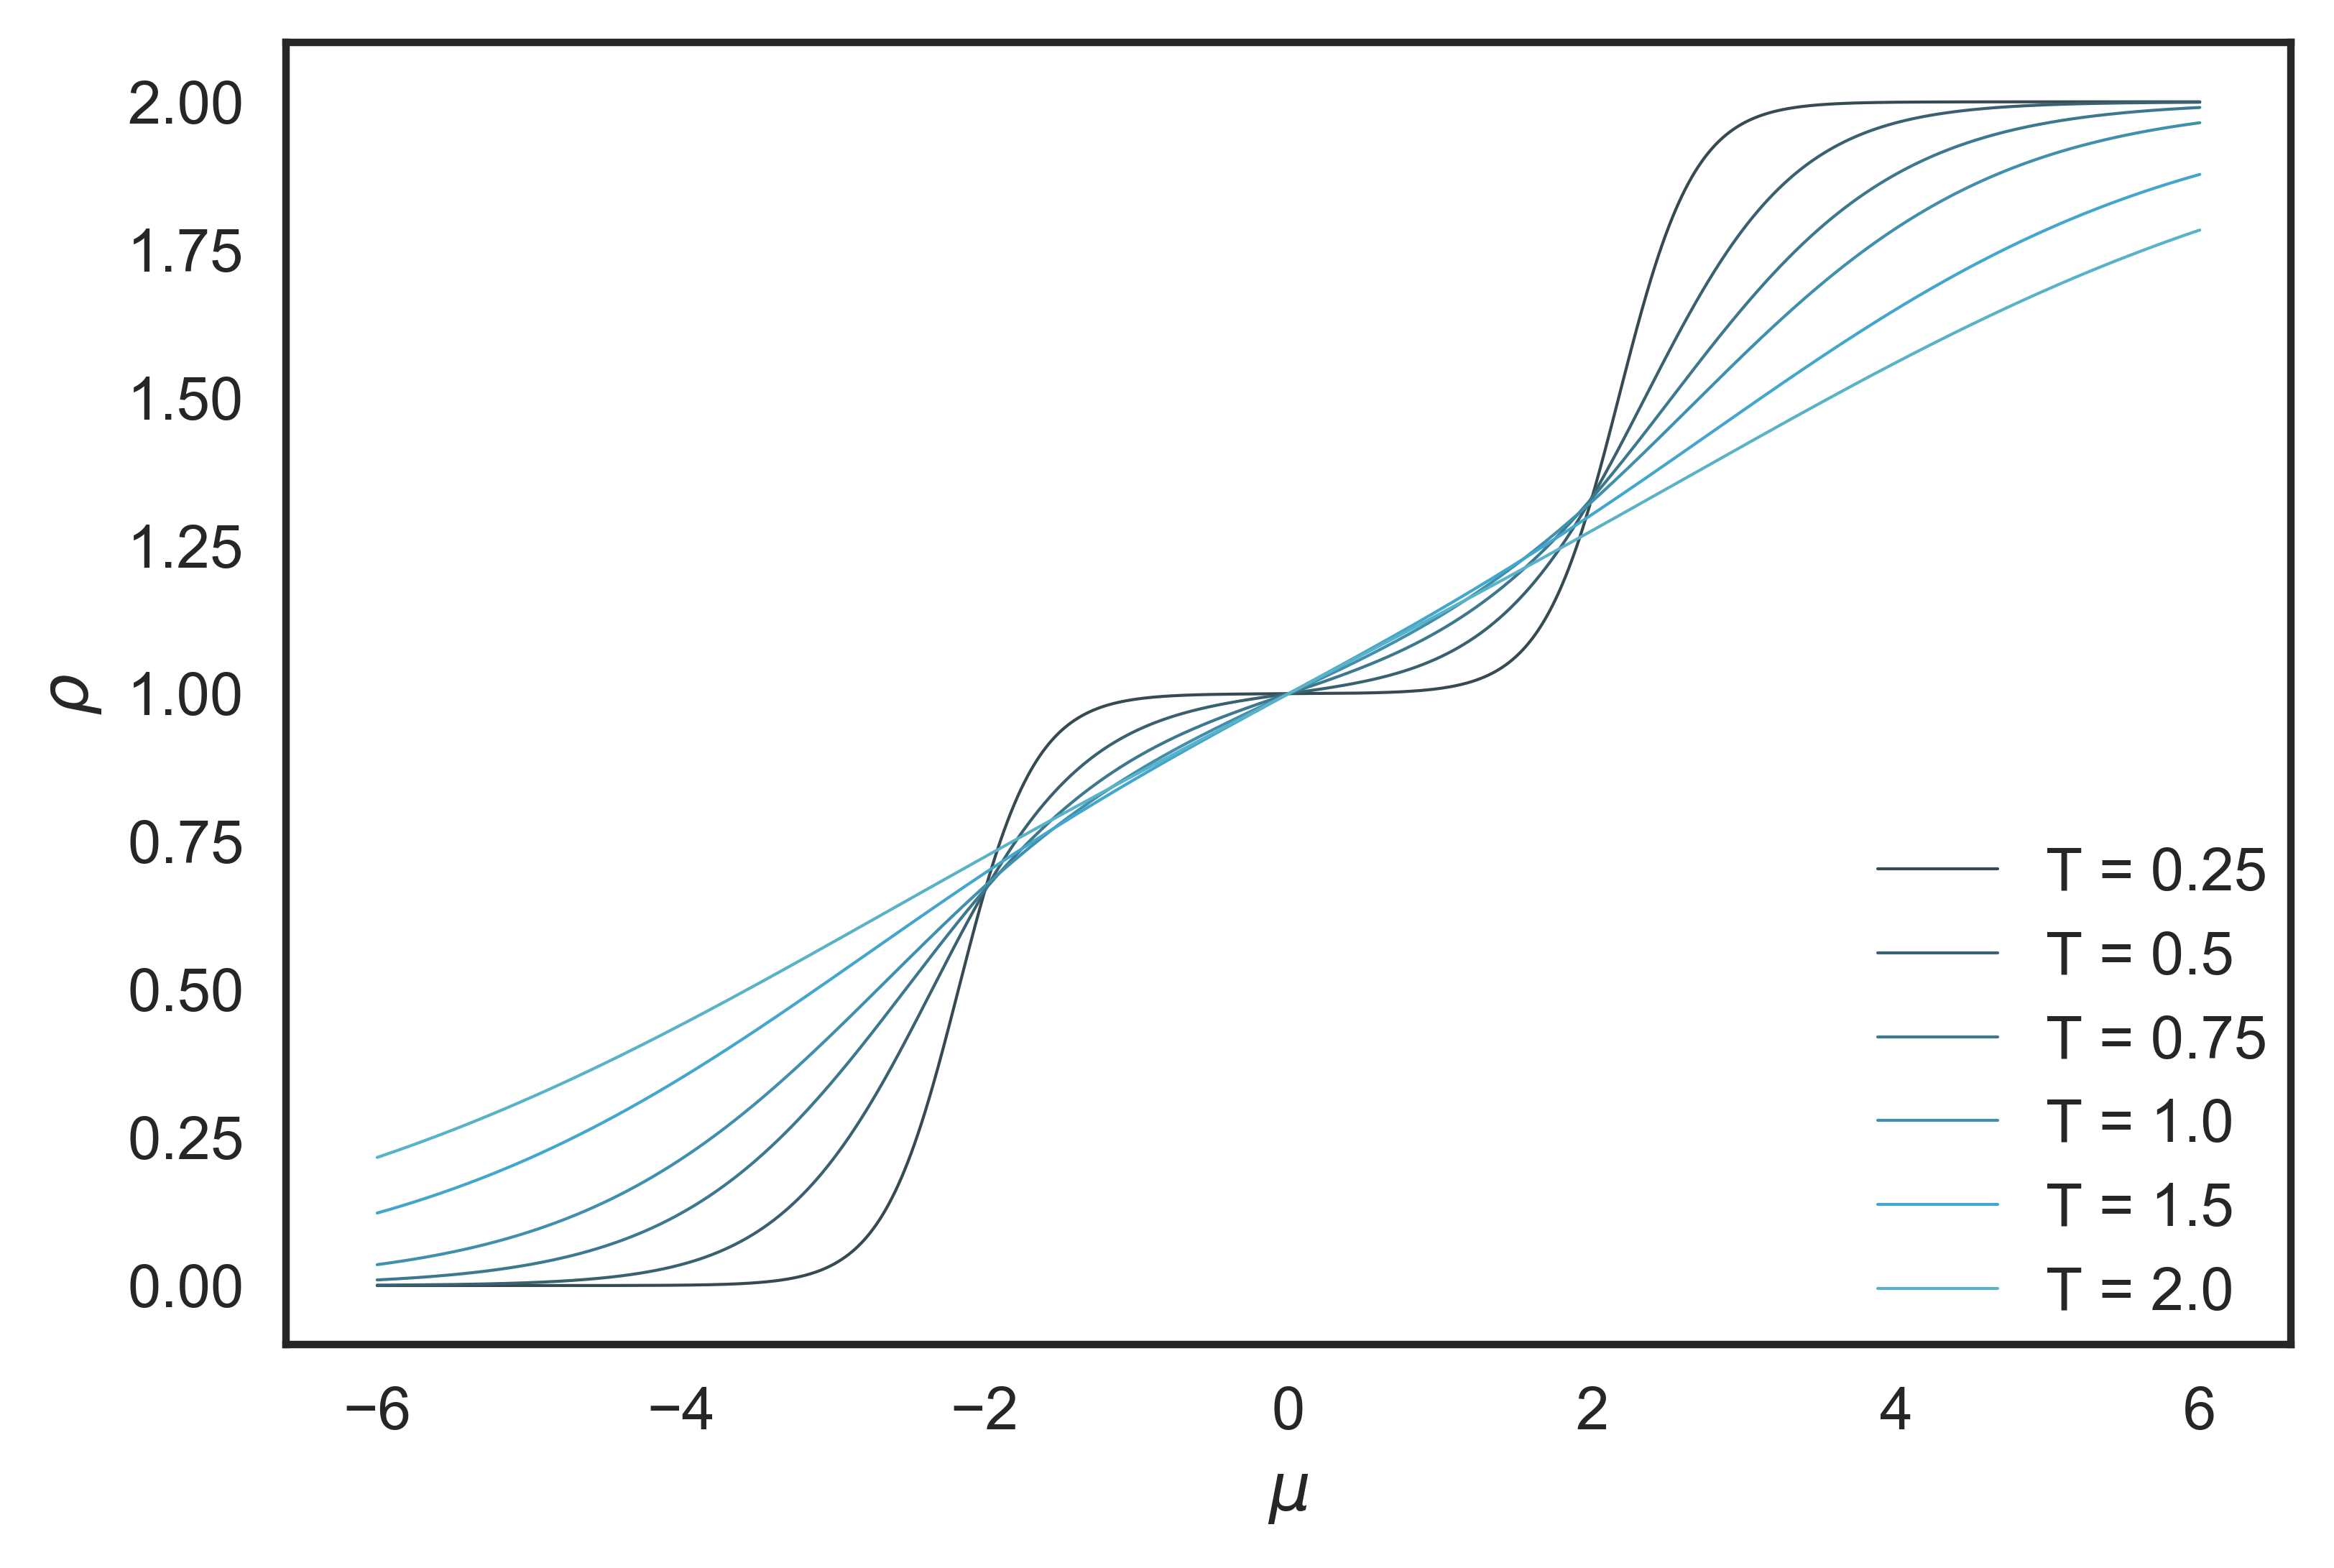
\includegraphics[width=0.7\linewidth]{Hubbard/rhoVsMu.png}
	\caption[Electron density in the purely atomic limit of the Hubbard model]{Electron density $\rho$ for varying chemical potential $\mu$ and temperature $T = \beta^{-1}$, but fixed $U = 4$. As the temperature decreases, a \say{Mott plateau} sets in. The Mott insulating gap already seen here is an important feature of the Hubbard model.}
	\label{fig:rhoVsMu}
\end{figure}

\item the one-site energy $E = \left\langle \mathcal{H} \right\rangle$.
\begin{equation}
\begin{split}
E &= \frac{\text{Tr}\bigg( \mathcal{H}e^{-\beta\mathcal{H} } \bigg)}{Z} = \frac{ \frac{U}{4} + 2 ( -\mu - \frac{U}{4} ) e^{\beta(\frac{U}{2} + \mu )} + (\frac{U}{4} - 2\mu ) e^{2\beta\mu}}{1 + 2 e^{\beta (\frac{U}{2} + \mu )} + e^{2\beta\mu} } \\
&= \frac{ \frac{U}{4} ( 1 + 2 e^{\beta (\frac{U}{2} + \mu )} + e^{2\beta\mu} )}{1 + 2 e^{\beta (\frac{U}{2} + \mu )} + e^{2\beta\mu} } + \frac{2(-\mu - \frac{U}{4}) e^{\beta(\frac{U}{2} + \mu)} - 2\mu e^{2\beta\mu} - 2\frac{U}{4} e^{\beta (\frac{U}{2} + \mu)} }{1 + 2 e^{\beta (\frac{U}{2} + \mu )} + e^{2\beta\mu}} \\
&= \frac{U}{4} - \frac{ (2\mu - U) e^{\beta(\frac{U}{2} + \mu) } + 2\mu e^{2\beta\mu} }{1 + 2 e^{\beta (\frac{U}{2} + \mu )} + e^{2\beta\mu} }
\end{split}
\end{equation}
which at half filling becomes

\begin{equation}
E = \frac{U}{4} - \frac{U}{2 ( 1 + e^{-\beta U /2} )}
\end{equation}

\item the double occupancy $\left\langle n_\uparrow n_\downarrow \right\rangle$.

\begin{equation}
\left\langle n_\uparrow n_\downarrow \right\rangle = \frac{\text{Tr} \big[ n_\uparrow n_\downarrow \big]}{Z} = \frac{e^{2\beta\mu}}{1 + 2 e^{\beta (\frac{U}{2} + \mu )} + e^{2\beta\mu}}
\end{equation}
which, at half filling, simplifies to

\begin{equation}
\left\langle n_\uparrow n_\downarrow \right\rangle = \frac{1}{2 ( 1 + e^{\beta U/2} )}
\end{equation}

Note that as either $U$ or $\beta$ increase the double occupancy tends to zero.
\end{enumerate}

As was motivated in the previous chapter, we are interested in studying magnetism in correlated systems.
For the Hubbard model, the relevant quantity is the local moment

\begin{equation}
\left\langle m^2 \right\rangle = \left\langle ( n_\uparrow - n_\downarrow )^2 \right\rangle = \left\langle n_\uparrow - n_\downarrow \right\rangle - 2  \left\langle n_\uparrow n_\downarrow \right\rangle = \rho - 2  \left\langle n_\uparrow n_\downarrow \right\rangle
\end{equation}

In figures (\ref{fig:mSqVsU}, \ref{fig:mSqVsT}), we show how $\left\langle m^2 \right\rangle$ varies as a function of $U$ for different temperatures, and how $\left\langle m^2 \right\rangle$ varies with $T$, for different values of the chemical potential, respectively.
At low temperature or for large on-site interaction, local moments tend to develop, which leads to magnetic ordering: $\left\langle m^2 \right\rangle \rightarrow 1$ (in the half-filled case).
Since the double occupancy is zero in this case, if we do not consider thermal fluctuations, the magnetization corresponds to the spin of the electron occupying the site.

\begin{figure}[H]
	\centering
\hspace{12mm}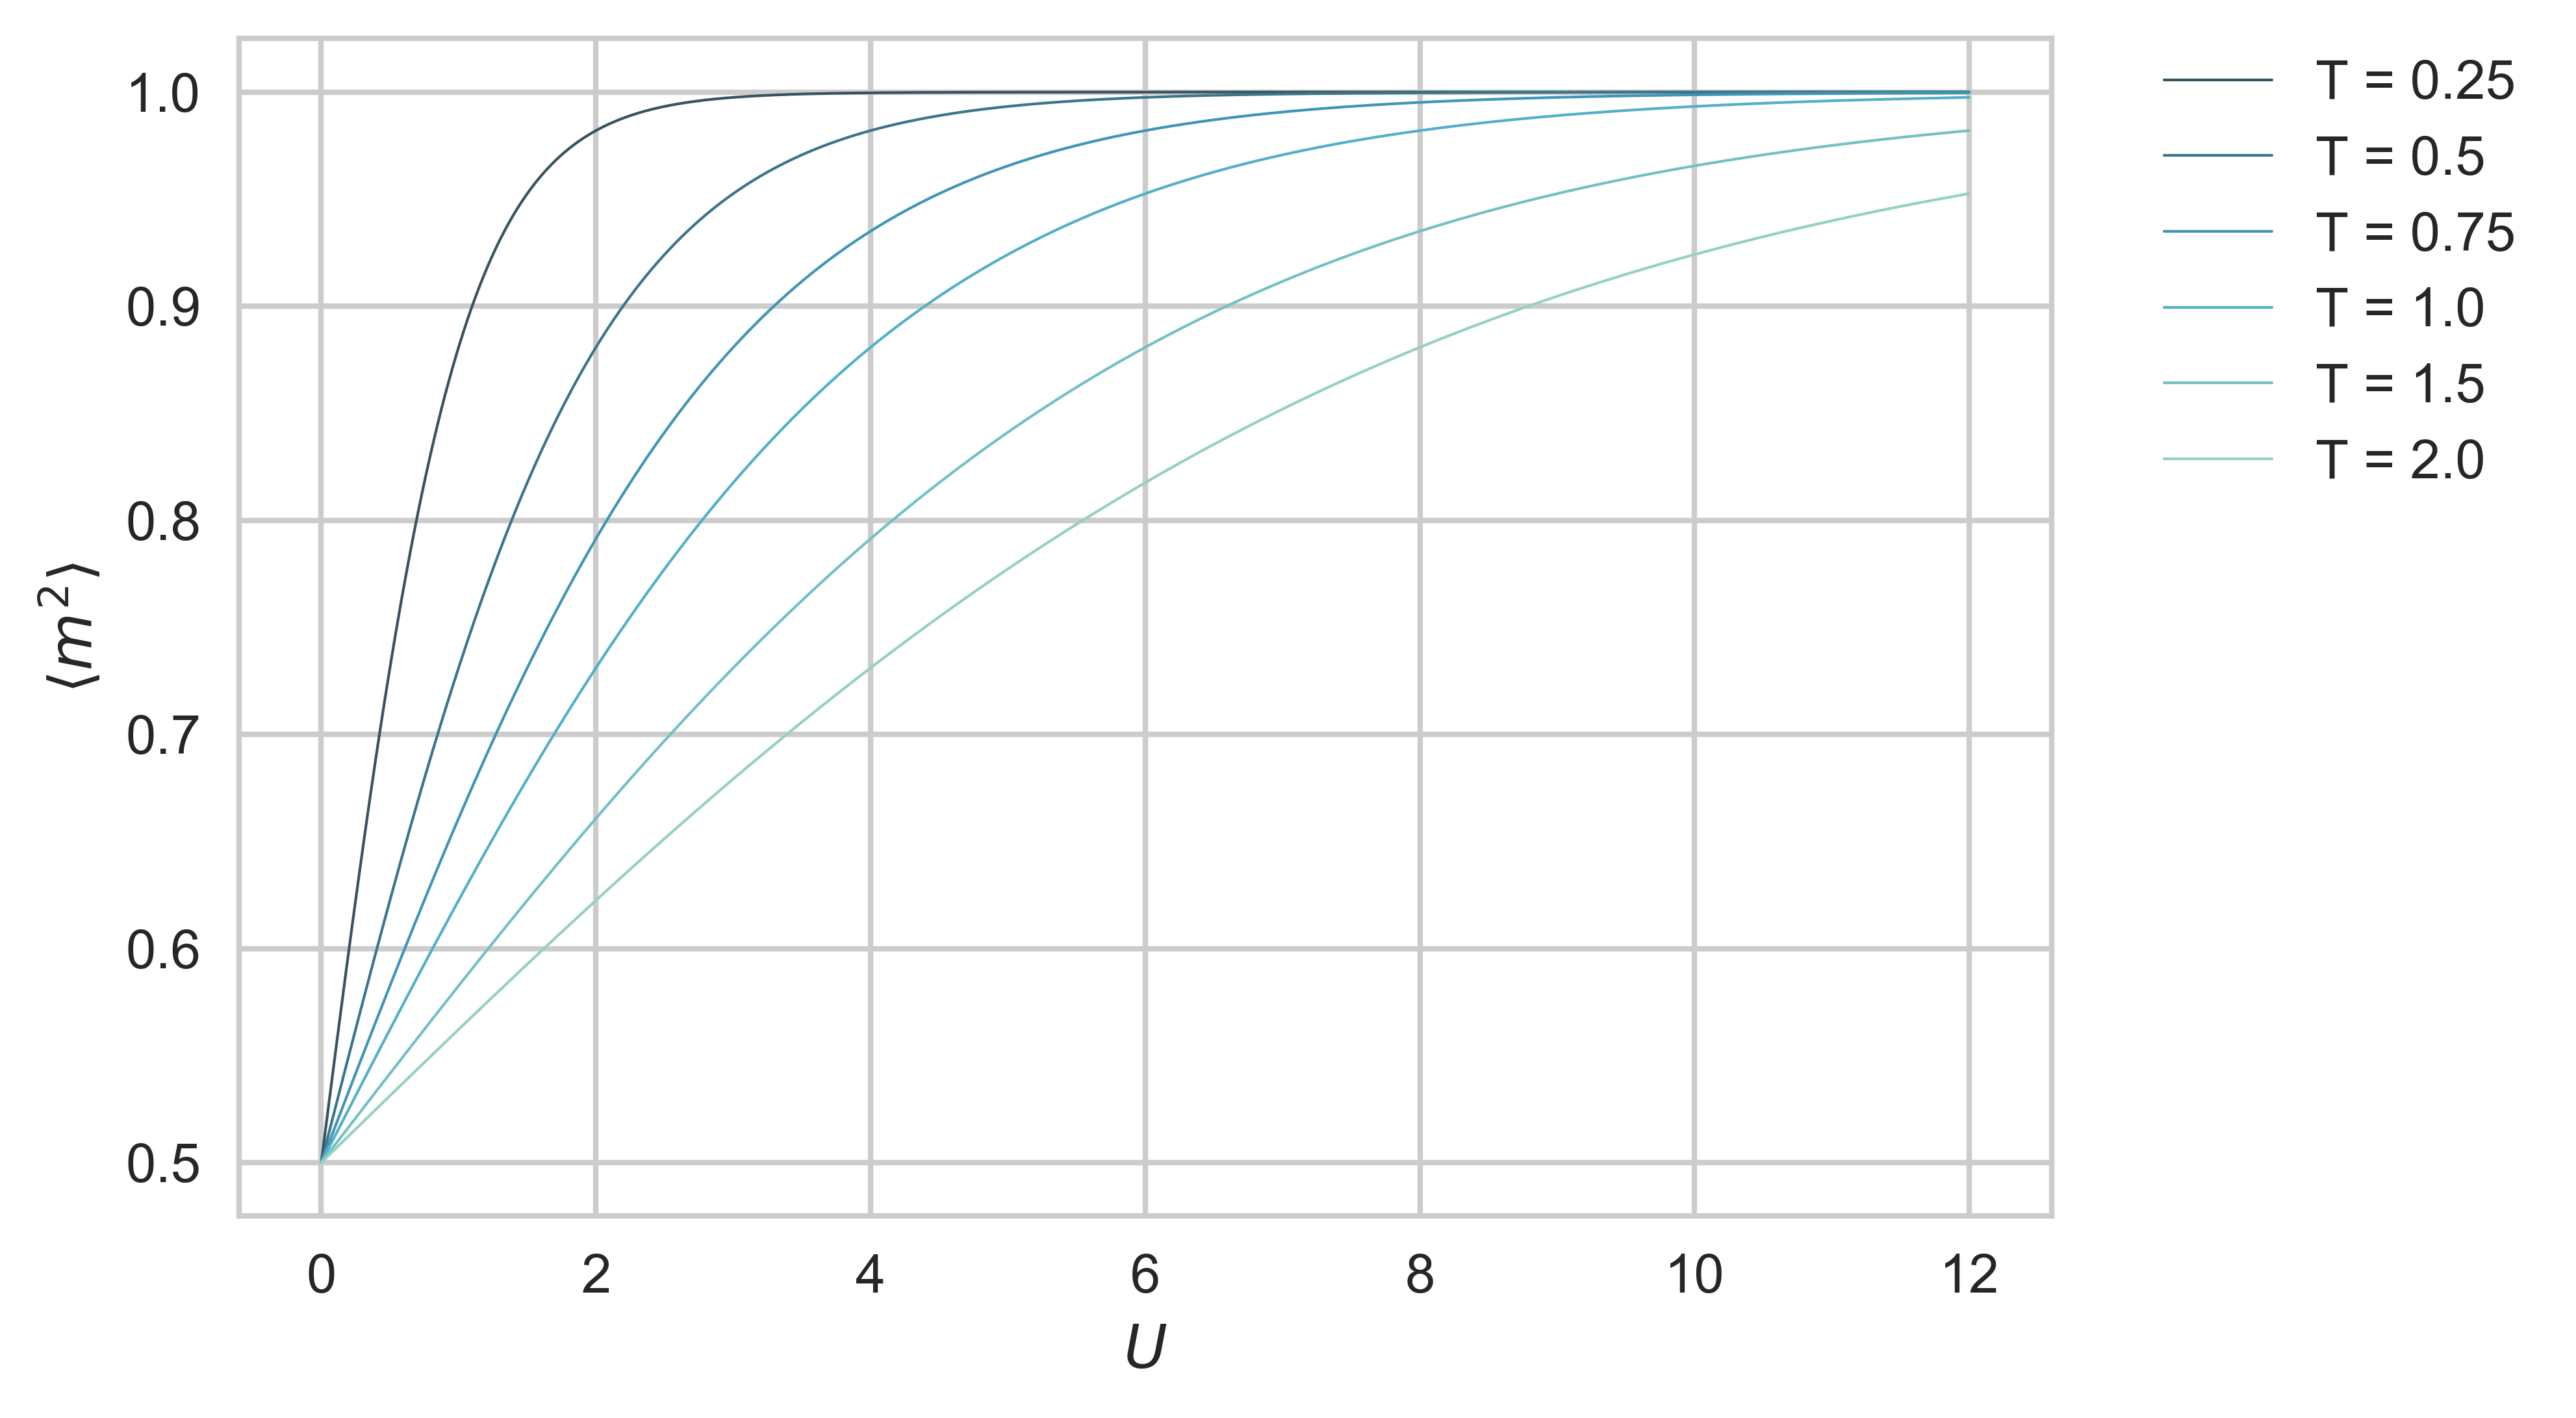
\includegraphics[width=0.7\linewidth]{Hubbard/mSqVsU.png}
	\caption[Magnetization as a function of the on-site interaction $\left\langle m^2 \right\rangle (U)$ in the single site Hubbard model for varying temperature $T$.]{Magnetization as a function of the on-site interaction $\left\langle m^2 \right\rangle (U)$ in the single site Hubbard model for varying temperature $T$.
	Local moments are favored by the on-site interaction, and are more likely to develop at lower temperatures, when thermal fluctuations are smaller. Here we consider half filling: $\mu = 0$.}
	\label{fig:mSqVsU}
\end{figure}

In figure(\ref{fig:mSqVsU}, we see thermal fluctuations destroying magnetic ordering.
As what happens for the Mott plateau, quantum fluctuations (i.e. introducing a hopping term in the Hamiltonian) change the behavior of the magnetization, and perfect moments ($\left\langle m^2 \right\rangle =1$) do not form anymore at zero temperature for finite on-site interaction.

\begin{figure}[H]
	\centering
\hspace{12mm}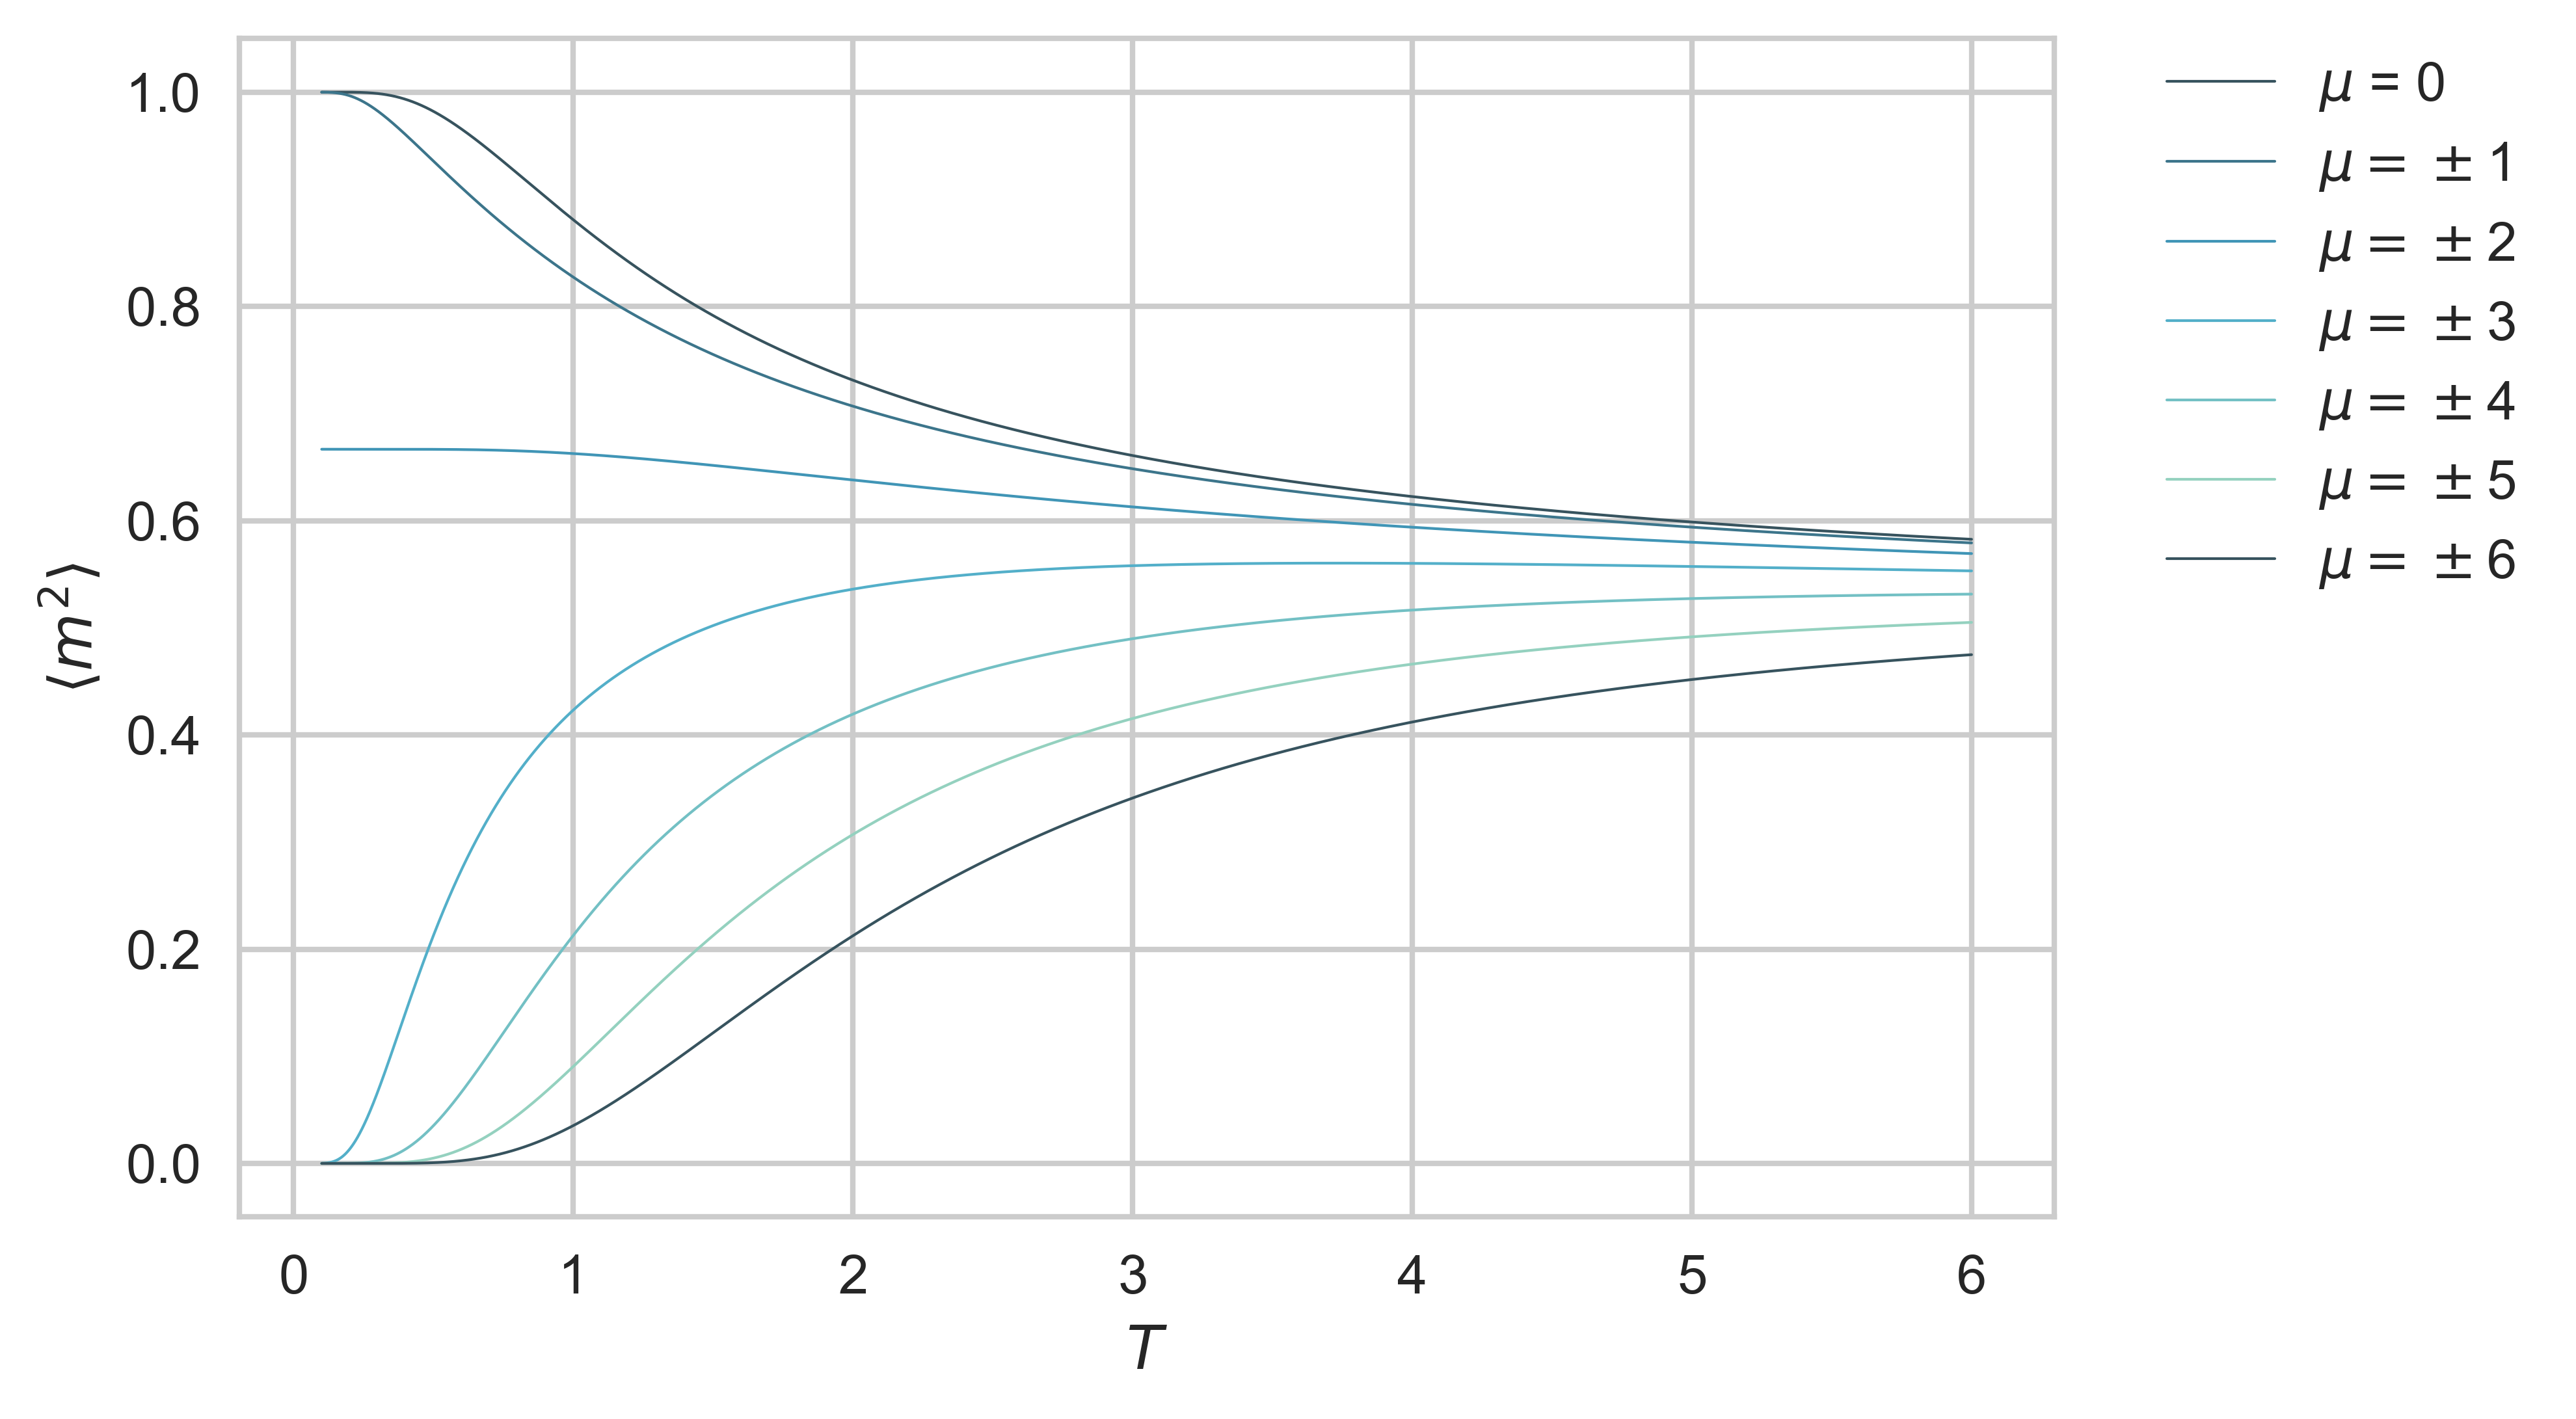
\includegraphics[width= 0.7\linewidth]{Hubbard/mSqVsT.png}
	\caption[Magnetization as a function of temperature $\left\langle m^2 \right\rangle (T)$ in the single site Hubbard model for varying chemical potential $\mu$.]{Magnetization as a function of temperature $\left\langle m^2 \right\rangle (T)$ in the single site Hubbard model for varying chemical potential $\mu$.
	Local moments develop at lower temperature.
	However, as we increase the chemical potential, the situation is reversed.
	At low temperatures, the site is doubly occupied and so the magnetization goes to zero.
	Thermal fluctuations allow the occupation of the site to fluctuate, and the magnetization to become nonzero.}
	\label{fig:mSqVsT}
\end{figure}

\subsection{The non-interacting $\frac{t}{U} \rightarrow \infty$ limit}

In the $\frac{t}{U} \rightarrow \infty$ limit, the spin sectors become independent, and they may be considered separately.
Thus, we omit the spin indices of the operators in the Hamiltonian:

\begin{equation}
\mathcal{H} = -t \sum_{\left\langle i, j \right\rangle} \bigg( c_i^\dagger c_j + c_j^\dagger c_i \bigg) - \mu \sum_i n_i = \bm c^\dagger \bigg( -t \bm K - \mu \bm I \bigg) \bm c ,
\end{equation}
where we casted the Hamiltonian as a bilinear form, and defined

\begin{equation}
\bm c = \bigg[ c_1 \,\, c_2 \,\, ... \,\, c_N \bigg]^T \quad \bm c^\dagger = \bigg[c_1^\dagger \,\, c_2^\dagger \,\, ... c_N^\dagger \bigg] ,
\end{equation}
and where $\bm I$ is the identity matrix.
We also defined a matrix of zeros and ones specifying the hopping geometry, $\bm K$. The elements of the hopping matrix are simply defined by the indicator function: $K_{ij} = \mathbbm{1}_{\left\langle j_i \right\rangle} (i)$, where $\left\langle j_i \right\rangle$ is the set of neighbors $j$ of site $i$.
When writing down $\bm K$, we must specify the boundary conditions.
\acp{PBC} preserve a system's translational invariance and are advantageous because they reduce finite size effects.
An example of a quantity which is measured more accurately is energy.
In the thermodynamic limit, $N \rightarrow \infty$, the measured energy differs from the actual value by a correction of order $\mathcal{O}(\frac{1}{N^2})$ with \acp{PBC}, while for \acp{OBC}, the correction is of order $\mathcal{O}(\frac{1}{N})$ \cite{hou_numerical_2009}.
Additionally, \acp{PBC} have the property of giving site independent observables.
For example, the electron density per site does not vary with the distance to the edges of the lattice with \acp{PBC}, but it does when we use \acp{OBC}.

For concreteness, let us consider a rectangular two-dimensional lattice with $N_x \times N_y$ sites. Then, we have $\dim(\bm K) = N_x N_y \times N_x N_y $, and

\begin{equation}
\bm K = \bm I_y \otimes \bm K_x + \bm I_x \otimes \bm K_y ,
\end{equation}
where $\bm I_{x, y}$ are identity matrices of dimension $N_{x, y} \times N_{x, y}$, respectively, and $\bm K_{x, y}$ are the hopping matrices in the $x$ and $y$-directions.

For lattices in \acs{1D} or \acs{2D}, it is possible to find an exact eigendecomposition

\begin{equation}
\bm K = \bm F^T \bm \Lambda \bm F \quad \text{with}  \quad \bm F^T \bm F = \bm I ,
\end{equation}
where $\bm \Lambda = \text{diag}(\lambda_{\bm k})$ is a diagonal matrix of eigenvalues of $\bm K$.
The Hamiltonian is diagonalized:

\begin{equation}\label{eq:quadraticH}
\mathcal{H} =\tilde{\bm c}^\dagger \big( -t \bm K - \mu \bm I \big) \tilde{\bm c} = \sum_{\bm k} \varepsilon_{\bm k} \tilde{n}_{\bm k} ,
\end{equation}
where $\tilde{\bm c} = \bm F \bm c$ and $\tilde{\bm c}^\dagger = (\bm F \bm c)^\dagger$, and

\begin{equation}
\varepsilon_{\bm k} = -t \lambda_{\bm k} - \mu \quad \tilde{n}_{\bm k} = \tilde{c}_{\bm k}^\dagger \tilde{c}_{\bm k}
\end{equation}

This is equivalent to performing a canonical transformation on the annihilation (creation) operators, that preserves not their Poisson brackets, as in classical mechanics, but their anti-commutators.
Finding the eigendecomposition is equivalent to changing to Fourier space:

\begin{equation}
\tilde{c}_{\bm k}^\dagger = \frac{1}{\sqrt{N}} \sum_{\bm j} e^{i \bm k \cdot \bm j} c_{\bm j}^\dagger ,
\end{equation}
a transformation which indeed preserves the anti-commutation relations, and the total number operator, i.e., $n = \sum_{\bm j} n_{\bm j} = \tilde{n} = \sum_{\bm k} n_{\bm k}$.

The $\tilde{c}$-operators are equally valid electron creation/annihilation operators, obeying the same anticommutation relations as the original operators $c_i$, and the total number operator is unchanged under our transformation
While the original operators create/annihilate particles at specific (spatial) sites, the new ones create/annihilate particles with momentum ${\bm k}$.
Both sets of operators describe the same physics.
Why can't procedure be applied to the interacting case?
For instance, the interaction term in the Hubbard model is fairly complex to write in momentum space so it is not possible to apply this procedure to diagonalize it.

Now, it turns out that it is easy to evaluate the partition function for quadratic Hamiltonians. If $\mathcal{H} = \bm c^\dagger \bm H \bm c$, where $\bm H$ is a $N \times N$ Hermitian matrix, then we have that

\begin{equation}\label{eq:trace_quadratic}
\text{Tr} \big[ e^{-\beta \mathcal{H} } \big] = \prod_{i=1}^N ( 1 + e^{-\beta \lambda_i } ) ,
\end{equation}
where $\lambda_i$ are the eigenvalues of $\bm H$. We present a proof of this result in appendix \ref{ap:Zquadratic}.

This result suggests that if we are able to devise some approximation to transform the quartic term of the interacting Hubbard model in a quadratic form, then we can solve it.
While this idea is essentially correct, the procedure is not straightforward.
Actually, we explore this in the next chapter to derive the simulation method that is at the basis of the entire thesis.

To complete the solution of the non-interacting case we apply the result of equation (\ref{eq:trace_quadratic}) to compute the partition function corresponding to the quadratic Hamiltonian defined in equation (\ref{eq:quadraticH}):

\begin{equation}
Z = \prod_{\bm k} ( 1 + e^{-\beta (\varepsilon_{\bm k} - \mu )} )
\end{equation}

Now that we have found a closed form solution for $Z$, it is again possible to find closed form expressions for observables of interest as well, namely:

\begin{enumerate}
\item the density, or average occupation of each site, $\rho$.

\begin{equation}
\rho = \left\langle n \right\rangle = \left\langle \tilde{n} \right\rangle = \frac{1}{N} \sum_{{\bm k}} \left\langle \tilde{n}_{\bm k} \right\rangle  = \frac{1}{N} \sum_{\bm k}  \frac{1}{1 + e^{\beta (\varepsilon_{\bm k} - \mu)}} = \frac{1}{N} \sum_{\bm k}  f_{\bm k}
\end{equation}

\item the energy $E = \left\langle \mathcal{H} \right\rangle$.
\begin{equation}
E = \frac{1}{N} \sum_{\bm k} \frac{\varepsilon_{\bm k} - \mu}{1 + e^{\beta(\varepsilon_{\bm k} - \mu)}} = \sum_{\bm k} (\varepsilon_{\bm k} - \mu) f_{\bm k}
\end{equation}

\item the equal-time Green's function, which plays a key role in computing other quantities, such as correlation functions.

\begin{equation}\label{eq:eqGreenNonInt}
G_{\bm l \bm j} = \left\langle c_{\bm l} c_{\bm j}^\dagger \right\rangle = \frac{1}{N} \sum_{\bm k} e^{ i {\bm k} \cdot ( \bm l -\bm  j ) } ( 1 - f_{\bm k} ),
\end{equation}
where $f_{\bm k} = \big(1 + e^{\beta(\varepsilon_{\bm k} - \mu)} \big)^{-1}$ is the Fermi-Dirac distribution (of course, here we consider half filling: $\mu = 0$).
Note that the Green's function, like the Hamiltonian, is translationally invariant: $G_{\bm l \bm j} = G_{\bm l-\bm j}$. 
If we use PBCs, no site is singled out, they are all equivalent and this behavior of the Green's function should become apparent in our simulations.
\end{enumerate}

The properties of a fermionic system are dominated by particles near the Fermi surface.
On the square lattice, a unique feature appears called perfect nesting. 
The wavevector $\bm k = (\pi , \pi)$ connects symmetric regions of the Fermi surface.
This suggests that this wavevector could have a crucial role in the description of the model in the square lattice.
Indeed, as we will see, a large magnetic structure factor at $\bm k = (\pi , \pi)$ signals antiferromagnetic order.
This is a feature of the Hubbard model at half filling down to $U = 0$.

\begin{figure}[H]
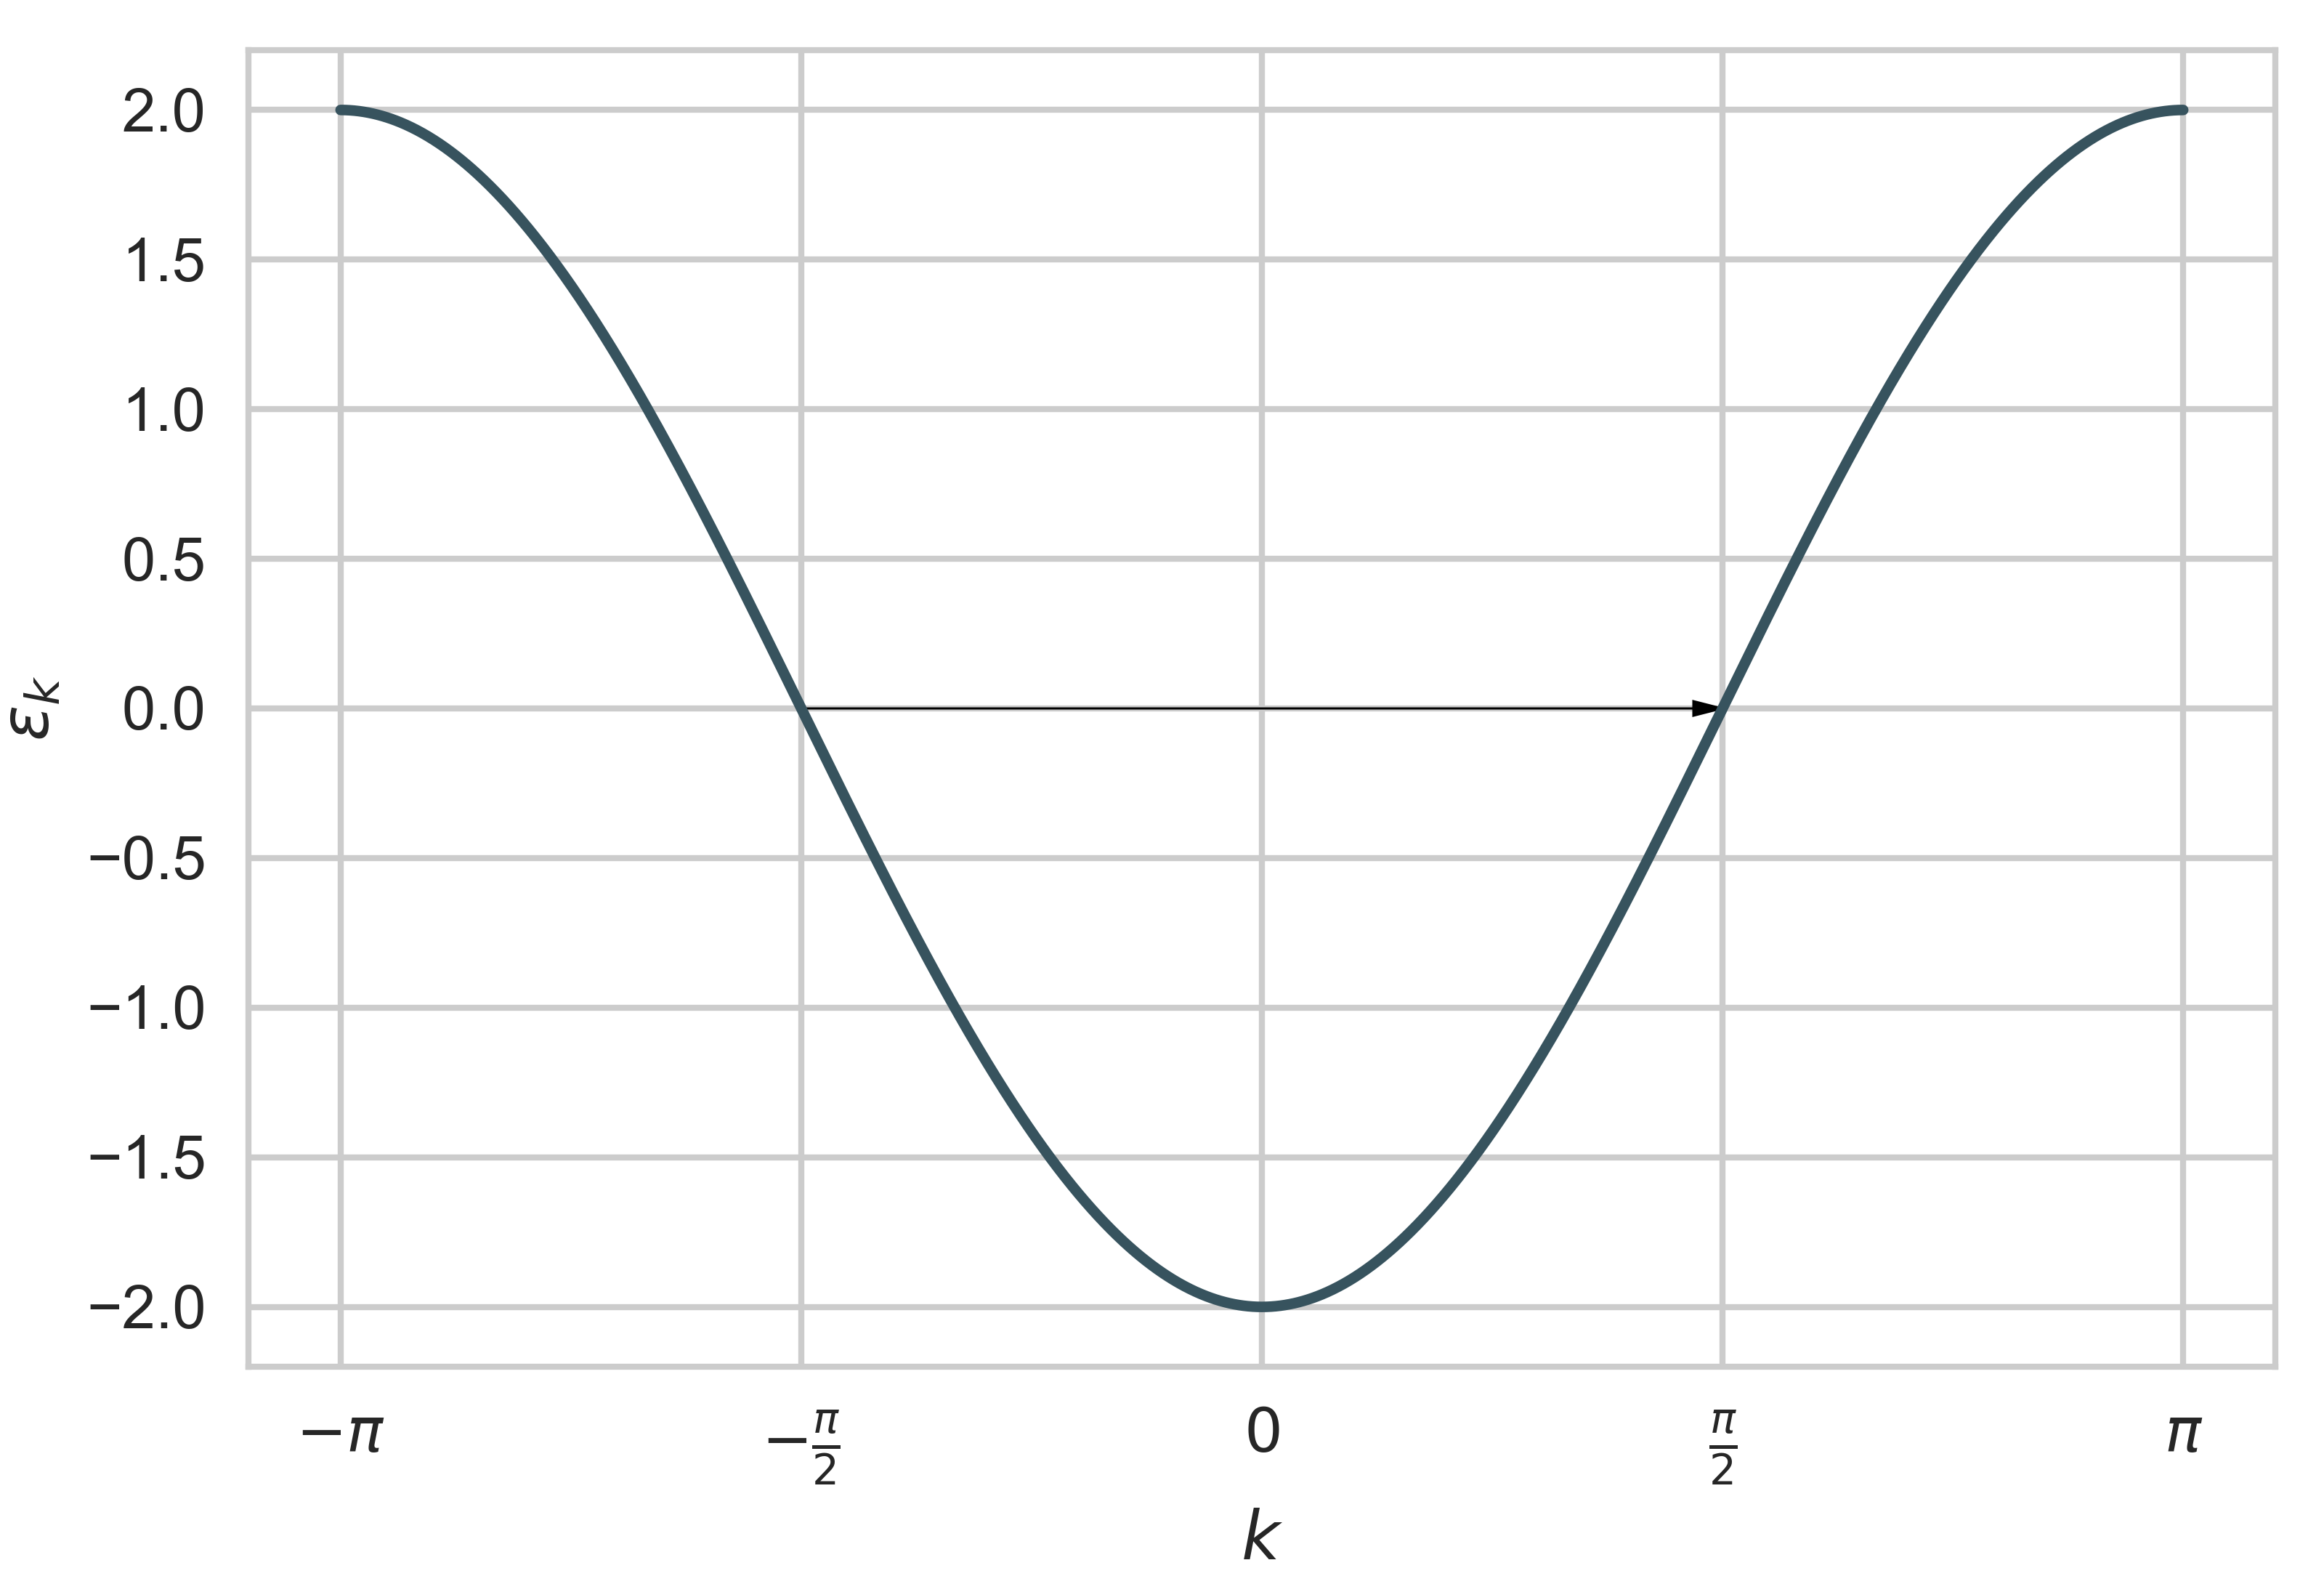
\includegraphics[width=0.55\linewidth]{Hubbard/fermiEnergy1D.png}
\hspace{-9mm}
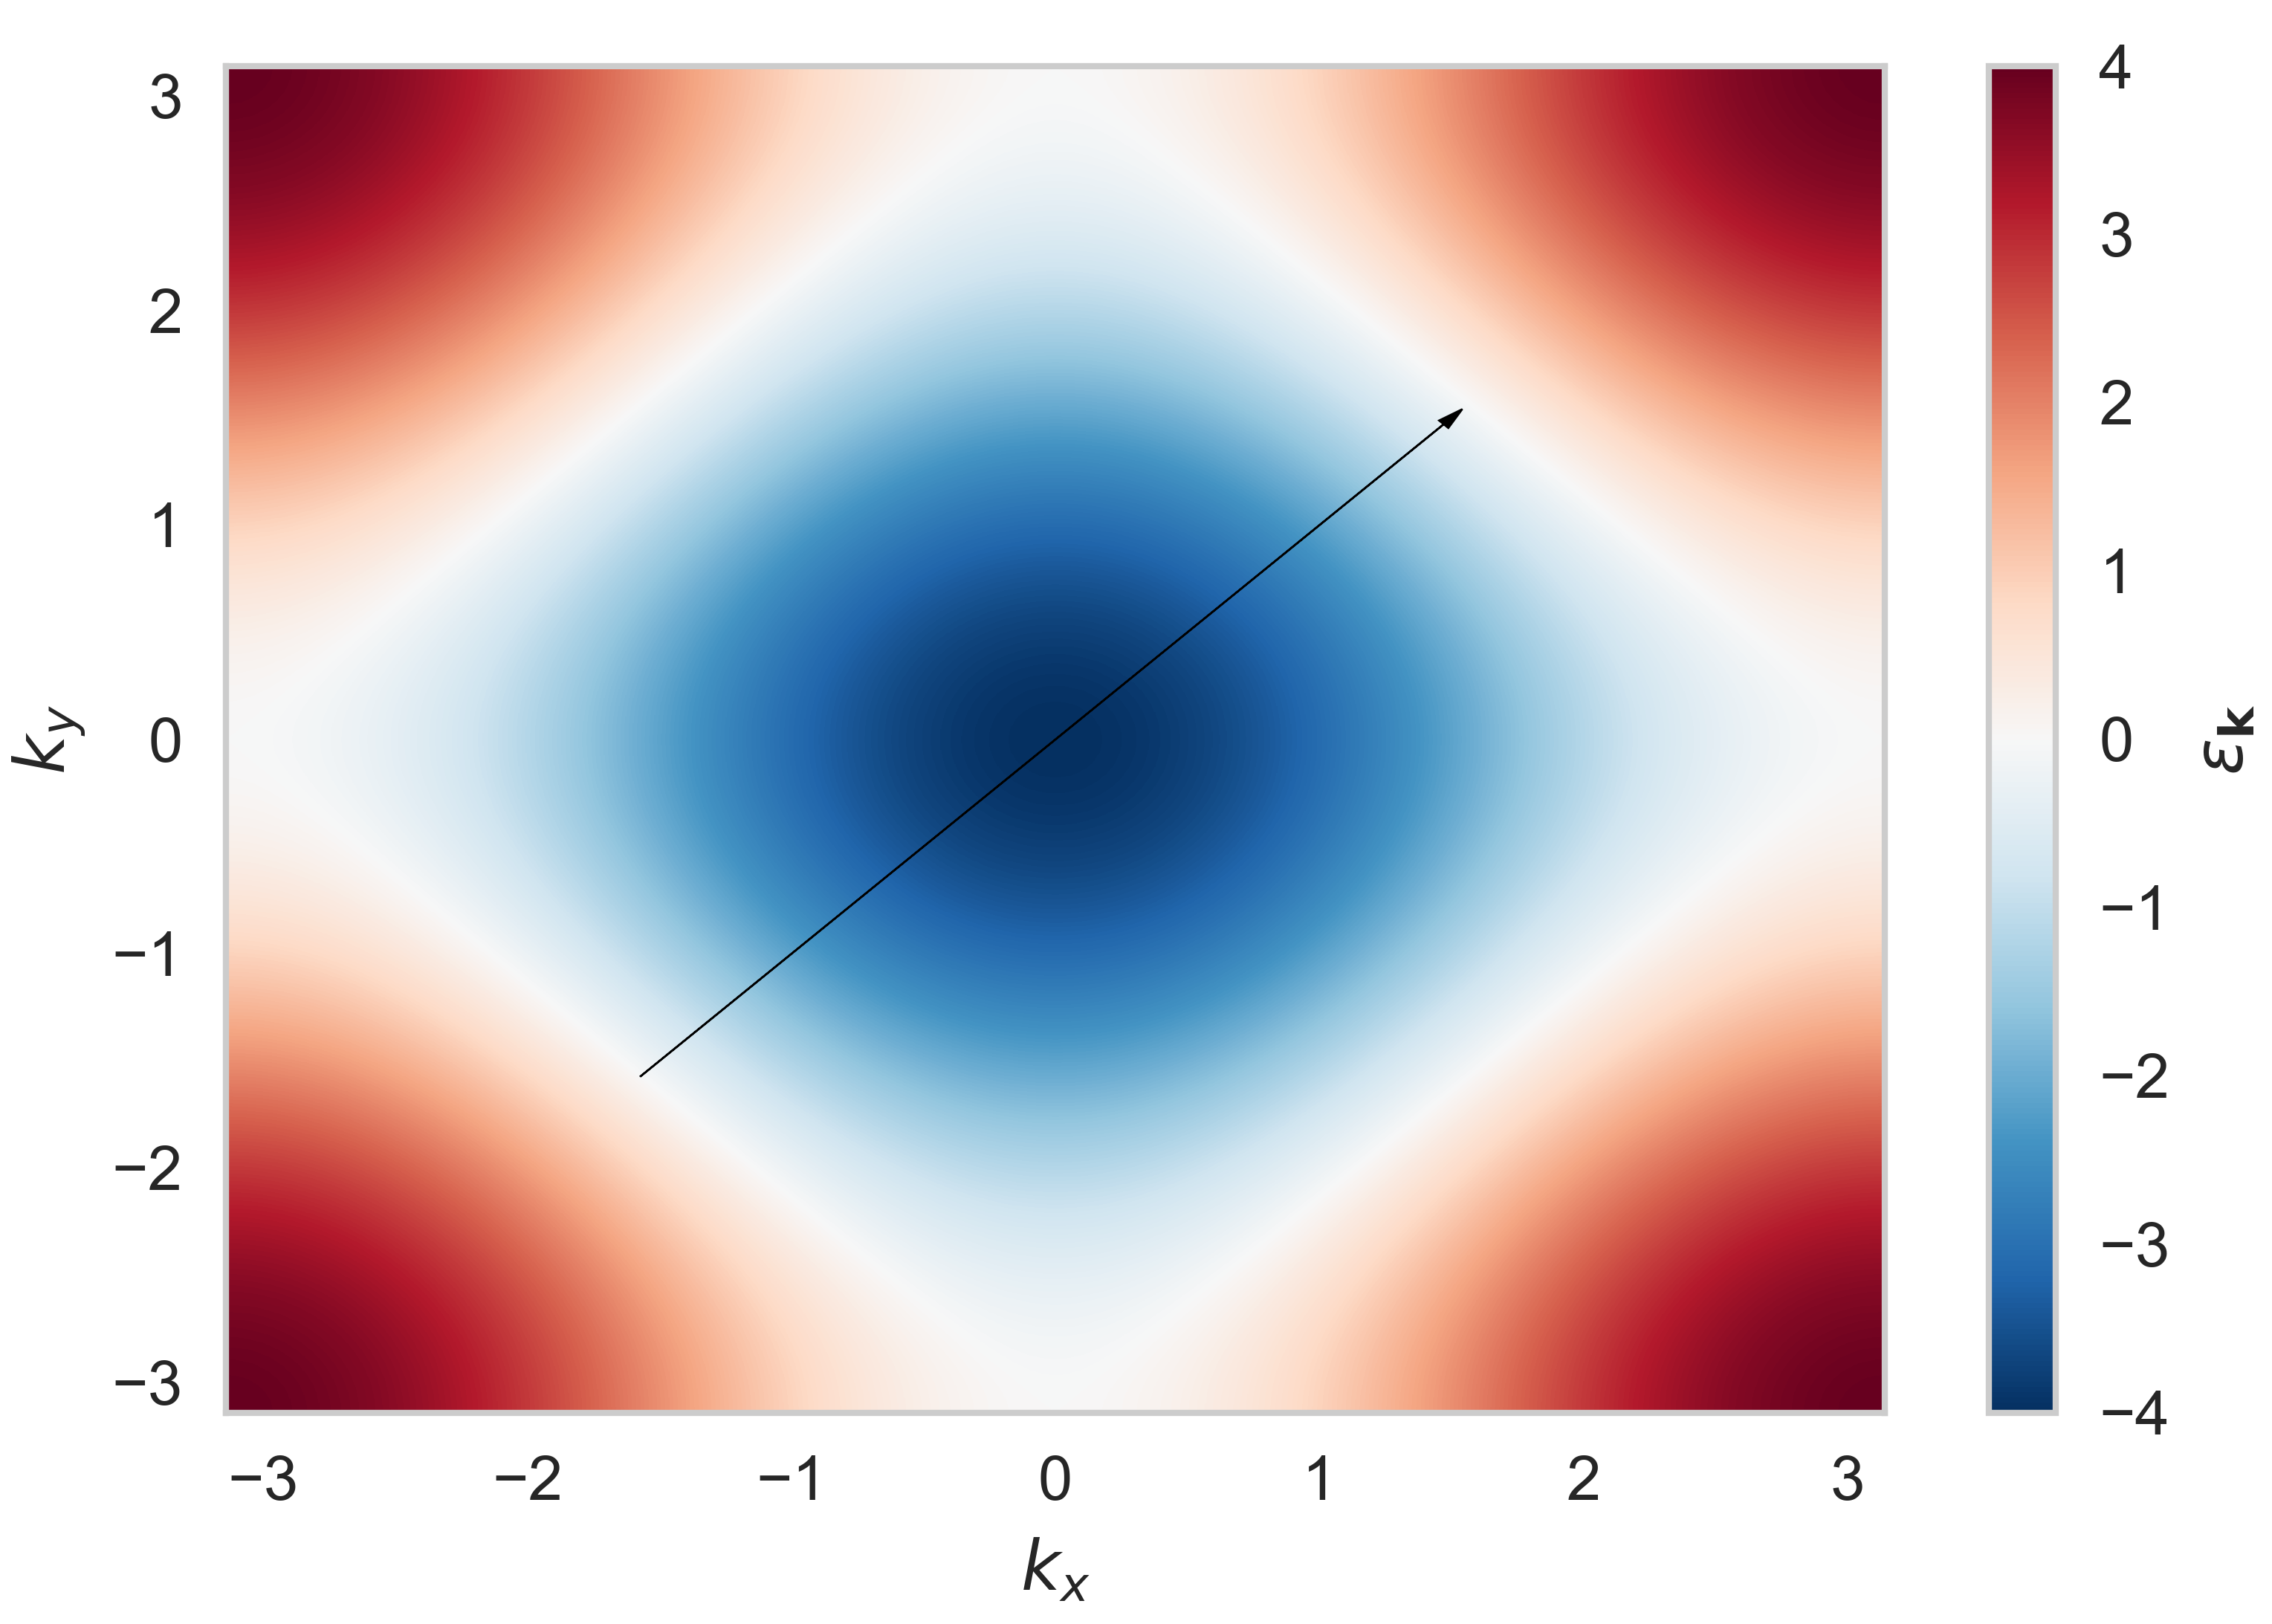
\includegraphics[width=0.49\linewidth]{Hubbard/fermiEnergy2D.png}
	\caption[Dispersion relations for the \acs{1D} chain and the square lattice in the non-interacting case.]{Dispersion relations for the \acs{1D} chain and the square lattice in the non-interacting case.
	For the square lattice, the surfaces separating the different colors are Fermi surfaces for different fillings of the lattice. In particular, for half filling ($\rho = 1, \mu = 0$, we obtain the rotated square in the white region.}
	\label{fig:fermi1D}
\end{figure}

From our analysis, we draw an important conclusion: that solving the single-particle problem, that is obtaining $\varepsilon_{\bm k}$ gives us all the information we need about all particle sectors (any number of particles, which is controlled via the chemical potential).
When the on-site interaction is \say{turned off}, the fermions simply occupy the one-particle states according to Pauli's exclusion principle.
The single-particle sector allows us to extrapolate to obtain the behavior of a system for any number of particles simply because $U = 0$; even if the hoppings were not uniform, this would hold.
The hoppings need not even be only between nearest neighbors, and in general we could even consider a chemical potential varying from site to site.
All we require is that the Hamiltonian is a quadratic form of the fermion operators.

\section{Effective $\frac{U}{t} \gg 1$ Heisenberg Model}\label{sec:effectiveHeisenberg}

In appendix \ref{ap:hubbardObSol}, we argue that Mott insulators allow low energy magnetic excitations (spin flips) without incurring into any energy cost whatsoever.
Their insulating phase corresponds to a configuration where each atom has an odd number of electrons, let's say one.
This electron may have its spin up or down.
In the purely atomic limit $\frac{U}{t} \rightarrow \infty$, the atoms are infinitely far, and the excitation spectrum is very simple.
The ground state is highly degenerate: every configuration with one electron per site is a ground state.
As a matter of fact, the ground state is $2^N$-fold degenerate.
The first excited state corresponds to configurations with a hole and a doubly occupied site.
Let us set the energy of the ground state to zero in our conventions.
The energy of these configurations is then $U$, and there are $N(N-1)2^{N-2}$ of them.
This process of generating higher energy excitations may be continued.
When the atoms are brought together, the first effect is the lifting of the degeneracy of the ground state, i.e. the splitting of the subspace of energy $E = 0$.
The effective Hamiltonian describing the lifting of the degeneracy of the lowest energy band is obtained by applying degenerate perturbation theory \cite{mila_physique_2007} to the kinetic term of the Hubbard Hamiltonian\footnote{An alternative method would be to use a canonical transformation technique.}
$
\mathcal{H}_0 = - t \sum_{\left\langle i, j \right\rangle, \sigma} ( c_{i\sigma}^\dagger c_{j\sigma} + c_{j\sigma}^\dagger c_{i\sigma} ) 
$.

\subsection{Two-site calculation}

The effect of the hopping term is best understood in a minimal two-site example.
There are four one-particle quantum states, represented by the action of the operators $c_{1,\uparrow}^\dagger$, $c_{1,\downarrow}^\dagger$, $c_{2,\uparrow}^\dagger$, $c_{2,\downarrow}^\dagger$ on the vacuum state.
There are six two-particle states in the Fock space represented by $\left| n_{1\uparrow} \,  n_{1\downarrow} \,  n_{2\uparrow} \, n_{2\downarrow} \right\rangle$:
\begin{equation}
\begin{split}
\left| 1 \right\rangle &\equiv \left| 1, 0, 1, 0 \right\rangle = c_{1\uparrow}^\dagger c_{2\uparrow}^\dagger \left| 0 \right\rangle \,\,\,\,
\left| 2 \right\rangle \equiv \left| 0, 1, 0, 1 \right\rangle = c_{1\downarrow}^\dagger c_{2\downarrow}^\dagger \left| 0 \right\rangle
\,\,\,
\left| 3 \right\rangle \equiv \left| 1, 0, 0, 1 \right\rangle = c_{1\uparrow}^\dagger c_{2\downarrow}^\dagger \left| 0 \right\rangle \\
\left| 4 \right\rangle &\equiv \left| 0, 1, 1, 0 \right\rangle = c_{1\downarrow}^\dagger c_{2\uparrow}^\dagger \left| 0 \right\rangle
\,\,\,
\left| 5 \right\rangle \equiv \left| 1, 1, 0, 0 \right\rangle = c_{1\uparrow}^\dagger c_{1\downarrow}^\dagger \left| 0 \right\rangle \,\,\,\,
\left| 6 \right\rangle \equiv \left| 0, 0, 1, 1 \right\rangle = c_{2\uparrow}^\dagger c_{2\downarrow}^\dagger \left| 0 \right\rangle \\
\end{split}
\end{equation}

The two-site Hamiltonian 
$
\mathcal{H}_{2} = - t \big( c_{1\uparrow}^\dagger c_{2\uparrow} +  c_{2\uparrow}^\dagger c_{1\uparrow} + c_{1\downarrow}^\dagger c_{2\downarrow} +  c_{2\downarrow}^\dagger c_{1\downarrow} \big) + U \big(n_{1\uparrow}n_{1\downarrow} + n_{2\uparrow}n_{2\downarrow} \big)
$ 
acts on the states of the Fock space as follows
\begin{equation}
\begin{split}
\mathcal{H}_{2}\left| 1 \right\rangle & = 0 \,\,
\mathcal{H}_{2}\left| 3 \right\rangle  =-t \big(c_{2\uparrow}^\dagger c_{1\uparrow} + c_{1\downarrow}^\dagger c_{2\downarrow} \big)c_{1\uparrow}^\dagger  c_{2\downarrow}^\dagger \left| 0 \right\rangle = -t \big( \left| 5 \right\rangle + \left| 6 \right\rangle \big)  \\
\mathcal{H}_{2}\left| 2 \right\rangle  &= 0 \,\,
\mathcal{H}_{2}\left| 4 \right\rangle =-t \big(c_{1\uparrow}^\dagger c_{2\uparrow} + c_{2\downarrow}^\dagger c_{1\downarrow} \big)c_{1\downarrow}^\dagger c_{2\uparrow}^\dagger \left| 0 \right\rangle = t \big( \left| 5 \right\rangle + \left| 6 \right\rangle \big) \\
\mathcal{H}_{2}\left| 5 \right\rangle & =\bigg[ -t \big(c_{2\uparrow}^\dagger c_{1\uparrow} + c_{2\downarrow}^\dagger c_{1\downarrow} \big) + U n_{1\uparrow}n_{1\downarrow}  \bigg]c_{1\uparrow}^\dagger c_{1\downarrow}^\dagger \left| 0 \right\rangle = U \left| 5 \right\rangle - t ( \left| 3 \right\rangle - \left| 4 \right\rangle )  \\
\mathcal{H}_{2}\left| 6 \right\rangle & = \bigg[ -t \big(c_{1\uparrow}^\dagger c_{2\uparrow} + c_{1\downarrow}^\dagger c_{2\downarrow} \big) + U n_{2\uparrow}n_{2\downarrow}  \bigg]c_{2\uparrow}^\dagger c_{2\downarrow}^\dagger \left| 0 \right\rangle = U \left| 6 \right\rangle - t ( \left| 3 \right\rangle - \left| 4 \right\rangle ) 
\end{split}
\end{equation}

When we act on the first two states we obtain $0$ because every term of the Hamiltonian gives a term $(c^\dagger)^2$, which is $0$ due to Pauli's exclusion principle.
The minus signs that appear on the hopping terms stem from the fermion anticommutation relations.

Let us now diagonalize the Hamiltonian in the subspace spanned by $\{\left| 3 \right\rangle, \left| 4 \right\rangle, \left| 5 \right\rangle, \left| 6 \right\rangle \}$.
If we add states $\left| 3 \right\rangle$ and $\left| 4 \right\rangle $, we get $0$ when acting with the Hamiltonian. 
$
\mathcal{H}_{2} ( \left| 3 \right\rangle + \left| 4 \right\rangle ) = 0
$.
On the other hand, if we subtract $\left| 5 \right\rangle$ and $\left| 6 \right\rangle$, we obtain
$
\mathcal{H}_{2}(\left| 5 \right\rangle -\left| 6 \right\rangle) = U( \left| 5 \right\rangle - \left| 6 \right\rangle)
$.
We have found two more eigenvalues (the first two were trivially found to be zero).
The others are found by subtracting $\left| 3 \right\rangle$ and $\left| 4 \right\rangle $ and adding $\left| 5 \right\rangle$ and $\left| 6 \right\rangle$: 
$\mathcal{H}_{2} ( \left| 3 \right\rangle + \left| 4 \right\rangle ) = -2 t  (\left| 5 \right\rangle + \left| 6 \right\rangle) \,\,
\mathcal{H}_{2}(\left| 5 \right\rangle -\left| 6 \right\rangle) = - 2 t (\left| 3 \right\rangle - \left| 4 \right\rangle ) + U (\left| 5 \right\rangle + \left| 6 \right\rangle) 
$.
The characteristic equation allowing us to find the rest of the eigenvalues in the rotated subspace spanned by $\{\left| 3 \right\rangle \pm \left| 4 \right\rangle, \left| 5 \right\rangle \pm \left| 6 \right\rangle  \}$ is
$
E ( E - U ) - 4 t^2 = 0 \iff E_{\pm} = \frac{1}{2} ( U \pm \sqrt{U^2 + 16 t^2} )
$.
Taylor expanding the square root up to second order, we obtain
$
E_- = -\frac{4t^2}{U} \quad E_+ = U + \frac{4t^2}{U}
$.
Thus, we have obtained the complete energy spectrum.
The ground state is a non-degenerate state of energy $-\frac{4t^2}{U}$, while the first excited state is a 3-fold degenerate state with energy $0$.
The two other excited states have energies of the order of $U$, the first one being exactly $U$ and the second $U + \frac{4t^2}{U}$.
There are four states for which the energy would be 0 if the hopping term vanished, corresponding to the four states with one electron per site.
The effect of the hopping term is to lift the degeneracy by splitting the 4-fold degenerate zero energy state into a singlet of energy $-\frac{4t^2}{U}$ and a triplet of energy $0$.
This is what we obtain my minimizing a Heisenberg Hamiltonian of the form
$
\mathcal{H}_{\text{Heis}} = \frac{4t^2}{U} \big( \bm S_1 \cdot \bm S_2 - \frac{1}{4} \big)
$
for two spins-$\frac{1}{2}$.
However, it turns out that this result is yet more general.
For an arbitrary number of sites, this is is the form of the effective Hamiltonian at second order (see appendix \ref{ap:hubbardObSol} for details).

It is easy to extend this analysis beyond half filling to compare it to our solution for the single site case.
The latter gave us some insight into how the on-site interaction gives rise to magnetic ordering, and about the development of the Mott plateau.
Adding in the hopping we can understand the interplay between kinetic and potential energy, and the magnetic correlations between sites.
In fact, we will outline the simplest nontrivial method to solve Hubbard-type Hamiltonians: \emph{exact diagonalization}, which is a competitor of \acs{QMC}, but is limited to very small system sizes.
Since the two-site Hamiltonian commutes with $n_\sigma$, it conserves the number of up and down fermions, and the $2^4 = 16$ states can be divided into 9 sectors of varying dimension $d$: $(n_\uparrow, n_\downarrow, d) = (0, 0, 1), (1, 0, 2),$
$ (2, 0, 1), (0, 1, 2), (1, 1, 4), (2, 1, 2), (0, 2, 1), (1, 2, 2), (2,2, 1)$.
There are four sectors of dimension 1: the empty and the fully filled lattices, and the lattices with two-like spin fermions.
All these sectors have zero kinetic energy: in the first, there are no electrons present to hop, and in the second Pauli's exclusion principle blocks hopping.
The sectors with $n_\sigma = 2$ have energy $- U / 2$, while the ones with $n_\uparrow = n_\downarrow$ have energy $U / 2$.

The four sectors of dimension 2 are also simple.
One and three particle sectors must have the same energy spectrum due to \acf{PHS}.
They have eigenenergies $\pm t$.
A single fermion can hop between sites, while out of the three fermions, the two with like-spin are blocked and can't hop to the same site, leaving a single fermion free to hop.
We have already solved the most complicated $n_\uparrow = n_\downarrow = 1$ sector, while tackling the half filled case.
By determining the complete spectrum of the two-site Hubbard model, we demonstrated that the eigenenergies in the $U \neq 0$ case can't be deduced solely from considering the single-particle sector.
The low temperature properties of the model are determined by the lowest energy eigenvalues, which all seem to fall in the half filled sectors.
Subtracting $U / 2$ to the energies we obtained in the half filled sectors is equivalent to considering the \acs{PHS} form of the Hamiltonian. 
At half filling, we end up with four states with energies around $-U / 2$ (the so called lower Hubbard band), and two states with energies around $U / 2$ (upper band).
The lower band controls the low temperature physics.
In the next section, we show that the Heisenberg Hamiltonian that seems to govern the behavior of the electrons in the lower Hubbard band is in fact the effective $U / t \gg 1$ model.

\subsection{Degenerate perturbation theory}

To first order in $\mathcal{H}$, the matrix elements of its effective Hamiltonian coincide in the ground state subspace, by definition:$
\left\langle m | \mathcal{H}_{\text{eff}} | n \right\rangle = \left\langle m | \mathcal{H}_0 | n \right\rangle ,
$ 
where $| m \rangle$, and $| n \rangle$ belong to the ground state subspace.
Since we are considering the system to be at half filling in our calculations, $| m\rangle$, and $| n \rangle$ must have one electron per site.
The hopping Hamiltonian $\mathcal{H}_0$ makes an electron hop, leaving its previous site empty, and the site it hops to doubly occupied.
This implies that to first order all the matrix elements are 0.

To second order, the matrix elements of the effective Hamiltonian are
\begin{equation}
\left \langle m | \mathcal{H}_{\text{eff}} | n \right\rangle = \sum_{ | k \rangle} \frac{\left\langle m | \mathcal{H}_0 | k \right\rangle \left\langle k | \mathcal{H}_0 | n \right\rangle }{E_0 - E_k} =-\frac{1}{U} \sum_{ | k \rangle} \left\langle m | \mathcal{H}_0 | k \right\rangle \left\langle k | \mathcal{H}_0 | n \right\rangle ,
\end{equation}
where $| k \rangle$ are the states that are not in the ground state subspace.
In the second equality we simply noted that $\mathcal{H}_0$ creates a doubly occupied site.
The energy cost of creating a doubly occupied site is $U$. 

In appendix \ref{ap:hubbardObSol}, we find the Heisenberg model as the effective Hamiltonian in this $\frac{U}{t} \gg 1$ limit.
This is consistent since the Heisenberg model couples spins on different sites, thus it is an \emph{atomic} model.
\begin{equation}
\mathcal{H}_{\text{eff}} = J \sum_{\left\langle i, j \right\rangle} \bm S_i \cdot \bm S_j ,
\end{equation}
with $J = 4 t^2 / U$.
Since $J > 0$, the model favors configurations with antiparallel adjacent spins.

There is an intuitive physical picture for this result: if two electrons on neighboring sites have parallel spins, none of the two can hop to the neighboring site due to Pauli's exclusion principle.
If adjacent sites have antiparallel spins, however, it is possible for any of the two electrons to hop to the neighboring site, and an exchange process allows the system to lower its energy.
First, a fermion hops to a neighboring site already occupied with an opposite spin fermion.
The intermediate state has a higher energy by $U$.
Then, the fermion hops back to its original site, in a process that decreases the energy by $E^{(2)} \propto - t^2 / U$.
\section{Green's functions and Wick's theorem}\label{sec:green}

Green's functions are the core of the first perturbative, diagrammatic approaches to the Hubbard model.
They are very useful in reducing the enormous amount of variables that come into play in correlated systems to a manageable number.
Here we try do give some intuition about how they work since they are the central quantity in the \acs{QMC} method we will use.
For a very complete and thorough description of the ideas in this section see \cite{fetter_quantum_2003}.

Considering the imaginary-time variable of the previous chapter $\tau = i t$, for $\tau > 0$, the Green's function is defined as

\begin{equation}
G_{\bm i \bm j} ( \tau, 0 ) = \left\langle c_{\bm i} ( \tau ) c_{\bm j}^\dagger ( 0 ) \right\rangle  \, , \text{with} \,\, c_{\bm i} ( \tau ) = e^{\mathcal{H} \tau } c_{\bm i} ( 0 ) e^{- \mathcal{H} \tau } 
\end{equation}

\subsection{Single site case}

The Hubbard Hamiltonian does not distinguish between spin-up and spin-down sectors.
Thus, without loss of generality, let us consider the spin-up sector, and compute $G_\uparrow (\tau, 0) =  \left\langle c_{\uparrow} ( \tau) c_{\uparrow}^\dagger ( 0 ) \right\rangle$.
Only the states $\left| n_{\uparrow} n_{\downarrow} \right\rangle = $ $\left| 0\, 0 \right\rangle$, $\left| 0\, 1 \right\rangle$ contribute to the expectation due to the creation operator on the right, which gives 0, unless there is no spin up electron already in the state it acts upon.

\begin{equation}
\begin{split}
c_{\uparrow} ( \tau) c_{\uparrow}^\dagger ( 0 )  \left| 0\, 0 \right\rangle &= e^{\mathcal{H} \tau } c_{\uparrow} ( 0 ) e^{-\mathcal{H} \tau } c_{\uparrow}^\dagger ( 0 )  \left| 0\, 0 \right\rangle = e^{\mathcal{H} \tau } c_{\uparrow} ( 0 ) e^{-\mathcal{H} \tau } \left| 0\, 1 \right\rangle \\
 &= e^{\mathcal{H} \tau } c_{\uparrow} ( 0 ) e^{U \tau / 4 + \mu \tau } \left| 1\, 0 \right\rangle = e^{\mathcal{H} \tau } e^{U \tau / 4 + \mu \tau } \left| 0\, 0 \right\rangle = e^{U \tau / 2 + \mu \tau } \left| 0\, 0 \right\rangle \\
 c_{\uparrow} ( \tau) c_{\uparrow}^\dagger ( 0 )  \left| 0\, 1 \right\rangle &= e^{\mathcal{H} \tau } c_{\uparrow} ( 0 ) e^{-\mathcal{H} \tau } c_{\uparrow}^\dagger ( 0 )  \left| 0\, 1 \right\rangle = e^{\mathcal{H} \tau } c_{\uparrow} ( 0 ) e^{-\mathcal{H} \tau } \left| 1\, 1 \right\rangle \\
 &= e^{\mathcal{H} \tau } c_{\uparrow} ( 0 ) e^{- U \tau / 4 + 2 \mu \tau } \left| 1\, 1 \right\rangle = e^{\mathcal{H} \tau } e^{- U \tau / 4 + 2 \mu \tau } \left| 0\, 1 \right\rangle = e^{U \tau / 2 + \mu \tau } \left| 0\, 1 \right\rangle
\end{split}
\end{equation}

Using the expression for the partition function that we obtained in equation (\ref{eq:singleSitePartition}), we arrive at

\begin{equation}
G_\uparrow (\tau, 0) = \frac{ e^{\tau ( U / 2 + \mu )} e^{-\beta U / 4} + e^{-\tau ( U / 2 - \mu )} e^{\beta (U / 4 + \mu)} }{ e^{-\beta U / 4} ( 1 + 2 e^{\beta ( U /2 + \mu)} + e^{2\beta \mu} ) } ,
\end{equation}
which, at half filling becomes

\begin{equation}
G_\uparrow (\tau, 0) = \frac{ e^{\tau U / 2} e^{-\beta U / 4} + e^{-\tau U / 2} e^{\beta U / 4 } }{ 2 e^{-\beta U / 4}  + 2 e^{\beta U / 4} } ,
\end{equation}

There is a well known relation between the Green's function and the spectral density $A ( \omega )$, which may be regarded as a local density of states:

\begin{equation}\label{eq:specDens}
G ( \tau, 0 ) =  \int_{-\infty}^{+\infty} A ( \omega ) \frac{e^{-\omega \tau} }{ e^{-\beta \omega} + 1 } d\omega ,
\end{equation}

If we replace the following expression for the spectral density in equation (\ref{eq:specDens}), we recover the result for the half filled case.

\begin{equation}
A ( \omega ) = \frac{1}{2} \bigg( \delta ( \omega - \frac{U}{2} ) + \delta ( \omega + \frac{U}{2} ) \bigg)
\end{equation}

We could do a similar calculation for $\mu \neq 0$ by changing the spectral density adequately, but the algebra is slightly more cumbersome, and the result does not bring additional insight.

The spectral density consists of two delta functions separated by $U$, which is reminiscent of our result for the Mott insulating gap.
In the same way that the gap softens (eventually disappearing) when we introduce hopping, the spectral function for the full Hubbard Hamiltonian changes accordingly, reflecting the same information about the properties of the system as the Green's function, encoded in a different manner.
In \acs{QMC}, we can access $G(\tau, 0)$ and deduce the properties of the system from it.

\subsection{Non-interacting case}

In this limit, we can compute $G_{\bm i \bm j} ( \tau, 0 )$ analytically by going to momentum space.

\begin{equation}
c_{\bm k} ( \tau ) = e^{ \mathcal{H} \tau } c_{\bm k} ( 0 ) e^{-\mathcal{H} \tau } = e^{-\varepsilon_{\bm k} \tau } c_{\bm k} ( 0 )
\end{equation}

This equation can be verified by acting with the left hand side and with right hand side on the states $\left| 0 \right\rangle$ and $\left| 1 \right\rangle$, and noting that the result is the same.
Alternatively, one can use the equation of motion $\partial_\tau \hat{A}(\tau) = [ \mathcal{H}, \hat{A} (\tau) ]$.
To generalize the result of equation (\ref{eq:eqGreenNonInt}) for the \emph{equal-time} Green's function to  \emph{unequal-time} we transform the fermionic operators in $G$ to momentum space, and use $\left\langle c_{\bm k} c_{\bm k}^\dagger \right\rangle = 1 - f_{\bm k}$ to obtain

\begin{equation}
G_{\bm i \bm j}(\tau, 0) = \frac{1}{N} \sum_{\bm k} e^{i \bm k \cdot (\bm i - \bm j )} ( 1 - f_{\bm k} ) e^{-\varepsilon_{\bm k} \tau } ,
\end{equation}
which is translationally invariant corresponding to the symmetry of the Hamiltionian.

We can generalize our definition of the Green's function by using the time-ordering operator $\mathcal{T}$:

\begin{equation}
G_{\bm k}(\tau, 0) = - \left\langle \mathcal{T} c_{\bm k} ( \tau) c_{\bm k}^\dagger ( 0 ) \right\rangle ,
\end{equation}
where

\begin{equation}
\mathcal{T} c_{\bm k} ( \tau) c_{\bm k}^\dagger ( 0 ) =
\begin{cases}
c_{\bm k} ( \tau) c_{\bm k}^\dagger ( 0 ), \,\, \tau > 0 \\
- c_{\bm k}^\dagger ( 0 ) c_{\bm k} ( \tau) , \,\, \tau < 0
\end{cases}
\end{equation}

An important property follows immediately from this definition: $G ( \tau + \beta, 0 ) = - G( \tau, 0 )$ for $ -\beta < \tau < 0$.
The imaginary-time periodicity constraint implies that the frequencies that appear when we Fourier transform are the so called (fermionic) Matsubara frequencies $\omega_n = \frac{(2n + 1) \pi}{\beta}$\footnote{Analogously, for bosons, imaginary-time anti-periodicity implies that $\omega_n = 2n \pi / \beta$}.

\begin{equation}
G ( i \omega_n ) = \int_0^\beta \frac{d\tau}{\beta} G( \tau, 0) e^{i\omega_n \tau} \quad\quad G (\tau) = \sum_n G ( i \omega_n ) e^{ - i \omega_n \tau}
\end{equation}

In momentum space, and imaginary time, the Green's function then become

\begin{equation}
G_{\bm k} (\tau, 0 ) =
\begin{cases}
-e^{-\varepsilon_{\bm k}} ( 1 - f_{\bm k} ) , \,\, 0 < \tau < \beta \\
e^{-\varepsilon_{\bm k}} f_{\bm k} , \,\, -\beta < \tau < 0 ,
\end{cases}
\end{equation}
which leads to

\begin{equation}
G_{\bm k} ( i \omega_n ) = \frac{1}{i\omega_n - \varepsilon_{\bm k} }
\end{equation}
in frequency space. This result may also be obtained by taking the partial derivative of the time-ordered Green's function written in the form $
G_{\bm k} ( \tau, 0 ) = \left\langle c_{\bm k} ( \tau) c_{\bm k}^\dagger ( 0 ) \right\rangle \theta ( \tau ) - \left\langle c_{\bm k} ( 0 ) c_{\bm k}^\dagger ( \tau ) \right\rangle \theta ( -\tau )
$
 and Fourier transforming both sides to solve for $G ( i \omega_n )$.
Taking a time derivative of $G$ implies computing commutators of $\mathcal{H}$ with the fermionic operators.
The equation closes for quadratic Hamiltonians, which we, of course, know to be soluble.

\subsection{Finite temperature Wick's theorem for fermions}
\label{subsec:wick}
\section{Magnetism and mean field theory}\label{sec:magMFT}

In this section we will build a picture of magnetism in the Hubbard model in increasing level of sophistication.
As our degenerate perturbation theory  calculation of section (\ref{sec:effectiveHeisenberg}) showed, the on-site interaction favors the situation in which neighboring fermions have opposite spins through an Heisenberg type interaction.
A different approach leads to the Stoner criterion for ferromagnetism.
The argument is based on creating an imbalance between the numbers of spin-up and spin-down fermions, and analyzing the interplay between the resulting increase in kinetic energy, and decrease in potential energy.
Finally, we formulate the Hubbard model in the mean field approximation, and discuss how it relates to the non-interacting case.

\subsection{Stoner criterion for ferromagnetism}
\label{subsec:stoner}

Pauli's exclusion principle gives a prescription on how to fill fermionic energy levels so as to yield the lowest possible total energy.
Start from the lowest level, and start filling each level of higher energy consecutively with two electrons, one of each spin.
This procedure requires the number of spin-up and spin-down electrons to be the same.
Otherwise, there is an energy cost, since we are obliged to fill higher energy levels with the excess electrons.
An unequal number of spin-up and spin-down electrons also decreases the potential energy.
An extreme example is a completely polarized lattice.
In that case, the potential energy is zero.
More generally, partial spin polarization makes double occupation unlikely, lowering the potential energy.

\begin{figure}[H]
	\centering
\hspace{12mm}\includegraphics[trim={0 7.5cm 0 7.5cm},clip, width=1 \linewidth]{Hubbard/dos.pdf}
	\caption[Density of states of the \acs{1D} tight-binding model.]{Density of states of the \acs{1D} tight-binding model.
	Here we represent a polarization of the spins, which leads to an increase in kinetic energy, since the imbalance of spins forces higher energy levels to be filled.}
	\label{fig:dos}
\end{figure}

A system with density of states $N(E)$ has equal densities of spin-up and spin-down electrons, $n$, filling the energy levels up to the Fermi energy, $\varepsilon_F$.
When we reduce, say the spin-up electron density by $\delta n$, the potential energy is lowered by $\delta P = U ( n + \delta n ) ( n - \delta n ) - U n^2 = - U (\delta n)^2$.

The extra density of electrons $\delta n$ that is added to the down sector will occupy levels with energy greater than $\varepsilon_F$, so that $\delta n = N ( \varepsilon_F ) \delta E$.
Some spin-up levels below $\varepsilon_F$ that used to be occupied are now empty, which makes $\delta n$ fermions per site increase their energy by $\delta E$, leading to a change in kinetic energy $\delta K = \delta n \delta E = \frac{(\delta n)^2}{N(\varepsilon_F)}$.
The global change in energy is

\begin{equation}
\delta E = \delta P + \delta K = \bigg( - U + \frac{1}{N(\varepsilon_F)} \bigg) \big( \delta n \big)^2 = \bigg( - U N ( \varepsilon_F ) + 1 \bigg) \frac{(\delta n)^2}{N(\varepsilon_F)}
\end{equation}

If $U N ( \varepsilon_F ) > 1$, then $\delta E < 0$, and the imbalance of spin densities actually becomes more favorable.
Thus, magnetism is favored by a large on-site interaction and a large density of states at (near) the Fermi energy.

\subsection{Mean field theory of the Hubbard model}

We have already encountered an example of a mean field theory when deriving the Hubbard Hamiltonian (see appendix \ref{ap:hubbardObSol}, where we provide motivation both heuristically and via a more rigorous variational approach).
In mean field theory, we give a systematic procedure to derive the most plausible quadratic Hamiltonian (which, as we know by now, is soluble) capturing some of the physics of our sytem.
We do this variationally in appendix \ref{ap:hubbardObSol}.
In the case of the Hubbard model, to find the best possible approximation for the quartic term we start by expressing the number operators in terms of an average plus fluctuations: $n = \left\langle n \right\rangle + ( n - \left\langle n \right\rangle ) \equiv \left\langle n \right\rangle + \delta n$.
Then, we make this substitution in the interaction term and neglect the term that is second order in the fluctuations to obtain

\begin{equation}\label{eq:meanFieldNop}
\begin{split}
n_\uparrow n_\downarrow &= \big( \left\langle n_\uparrow \right\rangle +  \delta n_\uparrow  \big) \big( \left\langle n_\downarrow \right\rangle +  \delta n_\downarrow  \big) = \left\langle n_\uparrow \right\rangle \left\langle n_\downarrow \right\rangle + \left\langle n_\downarrow \right\rangle ( n_\uparrow - \left\langle n_\uparrow \right\rangle ) + \left\langle n_\uparrow \right\rangle ( n_\downarrow - \left\langle n_\downarrow \right\rangle ) + \mathcal{O}((\delta n)^2) \\
&= n_\uparrow \left\langle n_\downarrow \right\rangle + n_\downarrow \left\langle n_\uparrow \right\rangle - \left\langle n_\uparrow \right\rangle \left\langle n_\downarrow \right\rangle
\end{split}
\end{equation}

We consider a \say{mean field} in the sense that the average density of spin-up electrons interacts with the spin-down electrons and vice-versa.
The last term subtracts the overcounted original single interaction term.
From equation (\ref{eq:meanFieldNop}), we obtain the quadratic mean field Hamiltonian

\begin{equation}
\mathcal{H}_{\text{MF}} = - t \sum_{\left\langle i, j \right\rangle, \sigma} \bigg( c_{i\sigma}^\dagger c_{j\sigma} + c_{j\sigma}^\dagger c_{i\sigma} \bigg) + U \sum_i \bigg( n_{i,\uparrow} \left\langle n_{i, \downarrow} \right\rangle + n_{i, \downarrow} \left\langle n_{i, \uparrow} \right\rangle - \left\langle n_{i, \uparrow} \right\rangle \left\langle n_{i, \downarrow} \right\rangle \bigg)
\end{equation}

To solve $\mathcal{H}_{\text{MF}}$, one merely has to diagonalize the corresponding matrix.
In the ferromagnetic case, the average occupation is independent of the specific site, but can vary with the spin species: $n_{i, \uparrow(\downarrow)} = n \Pm m$, where $m$ is the magnetization, the order parameter of the transition to a ferromagnetic phase.
Similarly, for the \acs{AF} case on a bipartite lattice, we consider $n_{i, \uparrow(\downarrow)} = n \Pm (-1)^{i} m$, leading to a staggered potential.

Now we take on a \acl{LG} theory kind of approach.
We compute the energy $E$ for fixed $n$ as a function of $m$, and inspect the system for ferromagnetic ordering: if the minimum lies at $m = 0$, the system is paramagnetic, otherwise it is ferromagnetic.
For simplicity, let us now consider the \acs{1D} model.
Since the average densities are site-independent, we can easily write down the polarized dispersion relations (up to an additive constant), and add these levels up for the various possible fillings of the lattice.

\begin{equation}\label{eq:meanFieldDispersion}
\varepsilon_{\uparrow k} = U ( n - m ) - 2 t \cos k \quad \varepsilon_{\downarrow k} = U ( n + m ) - 2 t \cos k ,
\end{equation}

The computational procedure to perfom mean field computations goes as follows:
\begin{itemize}
\item Fix the lattice size $N$, the total particle number $N_p$, and the on-site interaction $U$.
\item Set the possible densities by iterating $N_\uparrow = 0, 1, ..., N_p / 2$, and $N_\downarrow = N_p - N_\downarrow$ (we only need half the values since the values are symmetric under $ N_\uparrow \leftrightarrow N_\downarrow$), and setting $n_{\uparrow, \downarrow} = N_{\uparrow, \downarrow} / N$.
\item Fill the lowest $N_\uparrow$, and $N_\downarrow$ energy levels, by looping over the allowes momentum states $k = \frac{2\pi}{N} \{ -\frac{N}{2} + 1, -\frac{N}{2}, ..., \frac{N}{2} \}$, and using Eq.(\ref{eq:meanFieldDispersion}).
Normalize the energy to $N$ and add in the additive constant $- \left\langle n_\uparrow \right\rangle \left\langle n_\downarrow \right\rangle$.
This step is altered for the \acs{AF} case since we are assuming the up and down densities to be identical over the whole lattice.
In such case, we fix $n = N_p / 2$ and loop over $m = 1/ N, 2 / N,...$, staying within the first Brillouin zone.
Out of the energies computed in this way for varying $N_{\uparrow, \downarrow}$, the lowest gives the magnetization for the chosen values of $N_p$ and $U$.
\end{itemize}

\begin{figure}
	\centering
\hspace{12mm}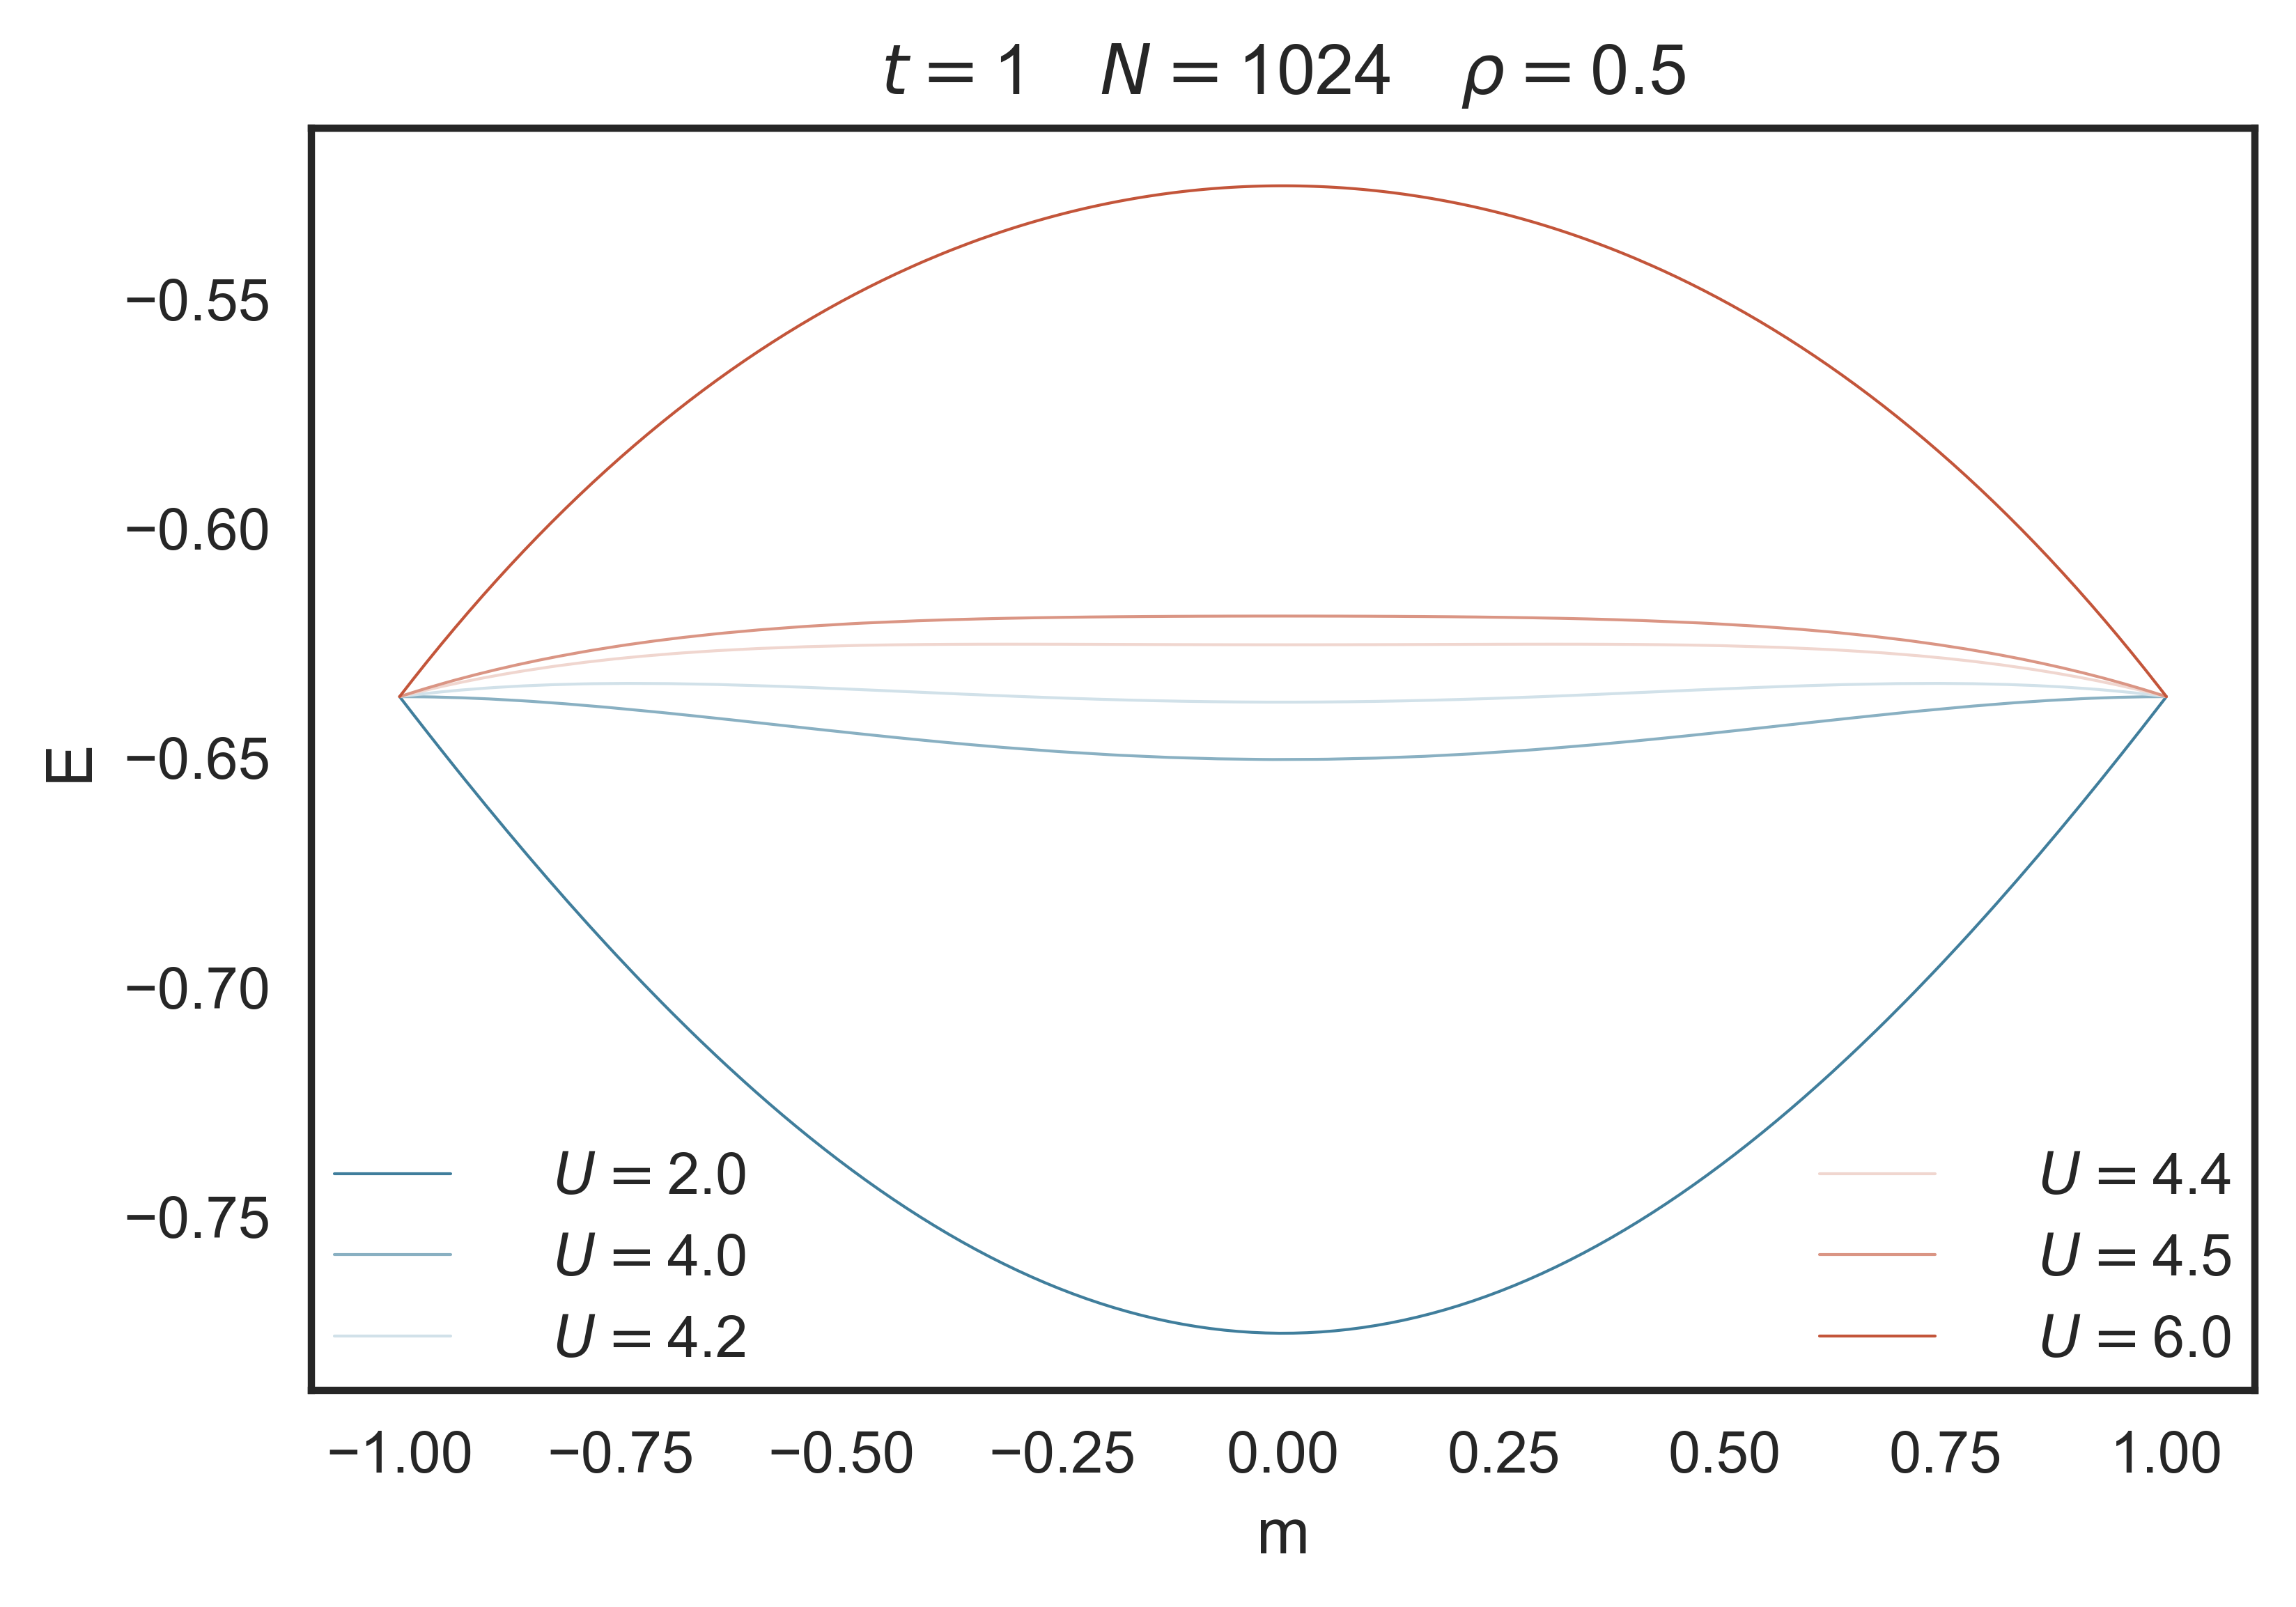
\includegraphics[trim={0 0 0 0},clip, width=0.6\linewidth]{Hubbard/mfHubbard.png}
	\caption[Mean field results for the \acs{1D} Hubbard model.]{Mean field results at quarter filling for a $ 1024$ sites chain.
	$U$ is in units of $t$.
	As the on-site interaction is increased, we see a transition from a paramagnetic to a ferromagnetic phase.}
	\label{fig:mft}
\end{figure}

\begin{figure}[H]
	\centering
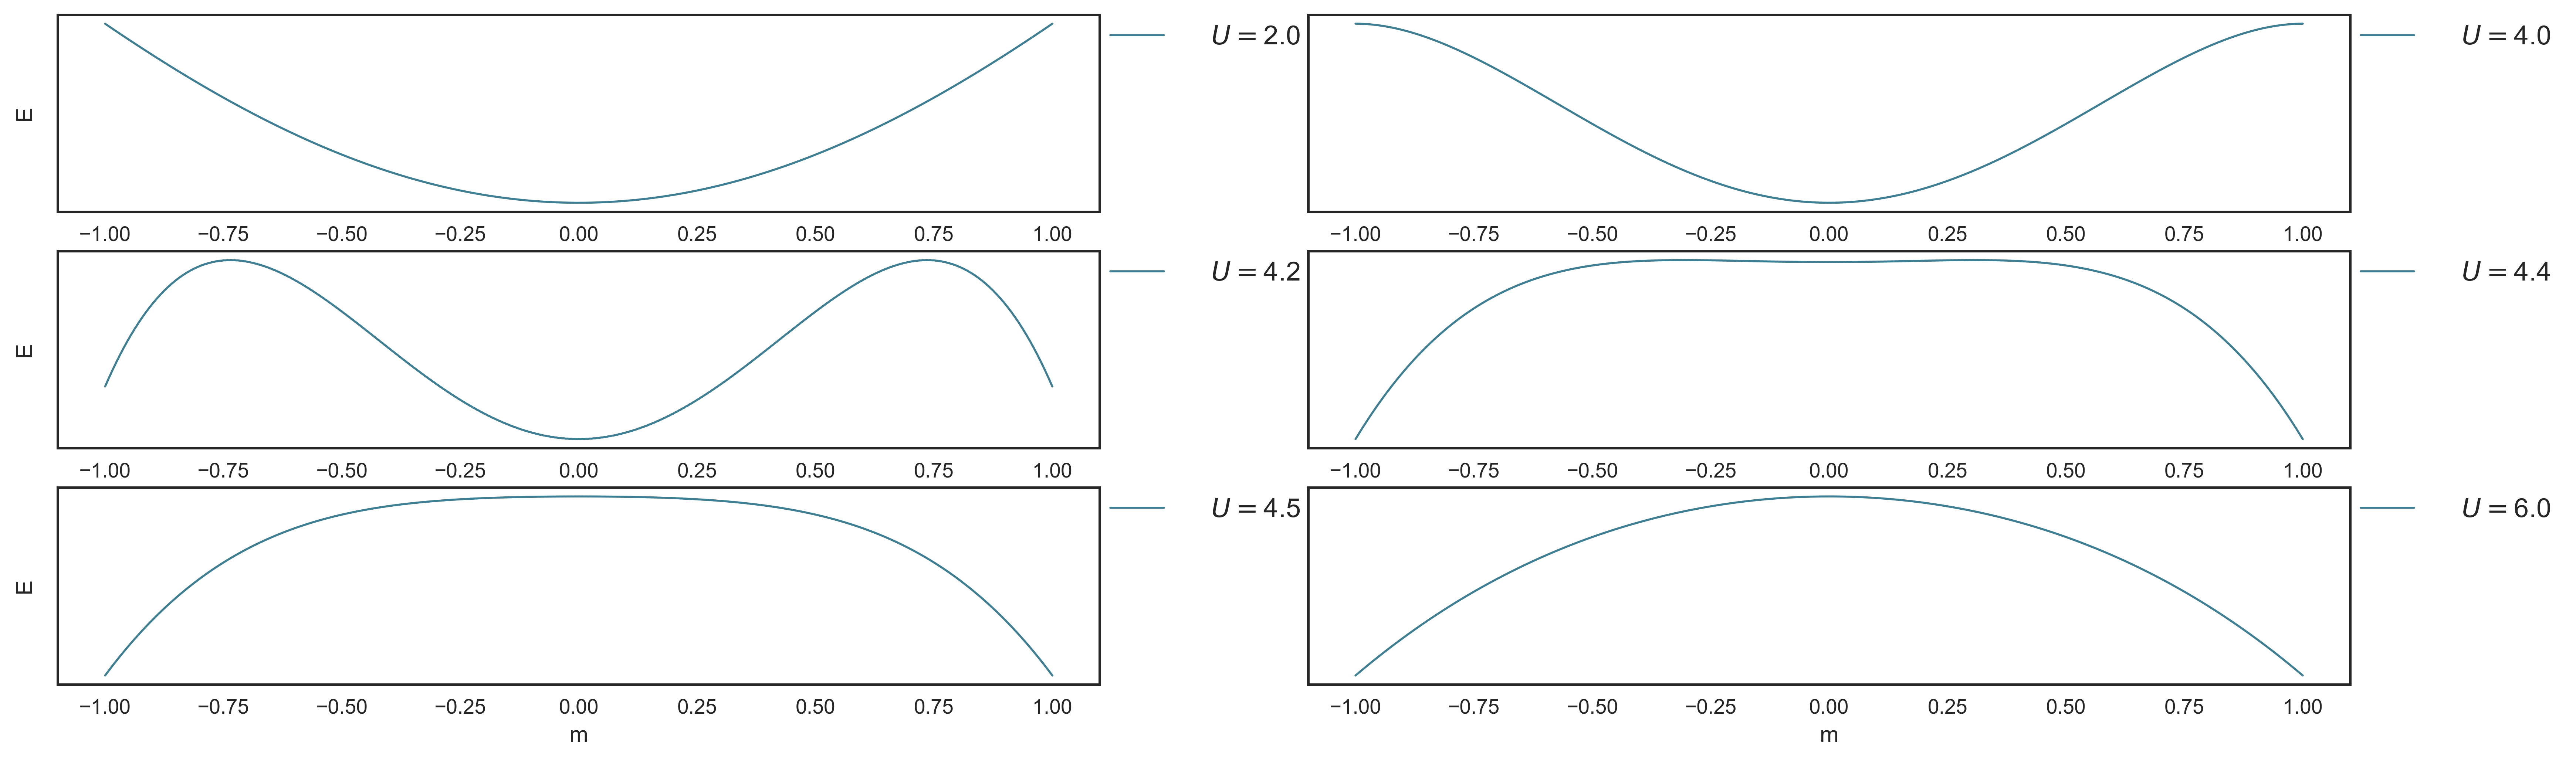
\includegraphics[trim={0 0 0 0},clip, scale = 0.3]{Hubbard/mfHubbard_multiple.png}
	\caption[Mean field results for the \acs{1D} Hubbard model: closing in on the phase transition.]{Plots of each energy curve separately giving evidence of a phase transition.
	}
	\label{fig:mft_multiple}
\end{figure}

Let us focus on Fig.(\ref{fig:mft_multiple}).
At $U = 2$, the phase is paramagnetic since the energy is minimized at $m = 0$. By $U = 4$, the phase transition is yet to occur but if you look at the energy scale in Fig.(\ref{fig:mft}), you will see that the energy of the spin polarized solutions decreased dramatically.
	At $U = 4.2$, the large $| m | $ energies have turned down, although $m = 0$ is still the lowest energy solution.
	At $U = 4.4$, the phase transition occurs, and the solutions with $| m | = 1$ become the lowest energy solutions: we have reached the ferromagnetic phase.

Are these results consistent with Stoner's criterion: $U N ( \varepsilon_F ) > 1$?
First, we use the density of states obtained in section (\ref{sec:exactSolutions}) to find a relation between the density $\rho$ and the Fermi energy $\varepsilon_F$:

\begin{equation}
\rho ( \varepsilon_F ) = 2 \int_{-2t}^{\varepsilon_F} dE N ( E ) \leadsto \rho_{\text{1D}} ( \varepsilon_F ) = \frac{2}{\pi} \arccos\bigg( \frac{-\varepsilon_F}{2t}\bigg) ,
\end{equation}
which behaves as expected, i.e. $\rho ( -2 t ) = 0$,  $\rho ( 0 ) = 1$, $\rho ( 2 t ) = 2$.
In terms of the electron density:

\begin{equation}
N ( \rho ) = \frac{1}{2\pi t \sin(\pi \rho / 2)} ,
\end{equation}
and in particular we can obtain the critical value $U_c$ at which the transition to the ferromagnetic phase takes place.
At quarter filling, we have $N( 1 / 2 ) = 1 /\sqrt{2} \pi t$, giving $U_c = \sqrt{2} \pi t \approx 4.44 t$, which is about what we obtained at the mean field level\footnote{Here, there can be finite size effects due to the finite size of the chain, $N = 1024$.}.

Mean field theory can be formulated in the \ac{GCE} as well.
One simply chooses the chemical potential $\mu$, and then computes $N_{\uparrow, \downarrow}$ by filling the levels below $\mu$.
The density is changed by tuning $\mu$.
In the \ac{GCE} case, the calculation is self-consistent, and is determined iteratively\footnote{One must pay attention so as not to get stuck in metastable states.}: the densities are updated until convergence occurs.
An example of the success of mean field is the discovery of striped phases of the Hubbard model, which are crucial in cuprate superconductors.
Recently, these phases have been probed by the \ac{QMC} method we shall use in this thesis \cite{huang_stripe_2018}.
In fact, mean field theory is insightful, but uncontrolled.
It tends to overestimate the possibility of ordering since it always predicts a phase transition.
Even if the transition does occur, generally its details are not perfectly captured (the critical temperature, the critical exponents, ...).

\subsection{Self-consistent solution in the \ac{GCE}}\label{subsec:selfconsistent}

In this section, we solve the mean field Hamiltonian in an iterative, self-consistent manner.

\begin{equation}
\mathcal{H}_{\text{MF}} = \mathcal{H}_\uparrow + \mathcal{H}_\downarrow + \mathcal{C} , \,\, \mathcal{H}_\sigma = - t \sum_{\left\langle i, j \right\rangle} \bigg( c_{i,\sigma}^\dagger c_{j,\sigma} + c_{j,\sigma}^\dagger c_{i,\sigma} \bigg) + U \sum_i n_{i,\sigma} \left\langle n_{i,-\sigma} \right\rangle , \,\, \mathcal{C} = - U \sum_i \left\langle n_{i,\uparrow} \right\rangle \left\langle n_{i,\downarrow} \right\rangle
\end{equation}

Since the interacting problem is turned into a single particle problem, the solution basically consists of diagonalizing two $N \times N$ matrices, where $N$ is the size of the system.
By varying the $2N$ mean field parameters, which are essentially the average local densities $\left\langle n_{i,\sigma} \right\rangle$, we can find the ground state, or other excited states, at the mean field level.
The mean field approach has several advantages: the Hilbert space is reduced from exponential to linear in the system size, which allows the study of relatively large systems; we can do the computation in real space; we can arbitrarily change the system geometry (introducing \acp{OBC}, defects, nonuniform hoppings); the model is flexible: tight-binding, and interaction terms are easily added to the Hamiltonian.
However, $SU(2)$ symmetry is broken, and electron correlations are neglected.
Only long range order is captured and its stability is often overestimated.
While the mean field solution approaches the exact solution at weak coupling $U$, it can give only qualitative behavior at best, when $U$ increases significantly.

The iterative method starts with the initialization of the mean field parameters.
This initial condition cannot be completely arbitrary because it affects convergence.
Typical choices are the random initial condition or the paramagnetic state.

Then, we repeat the following steps until convergence:

\begin{itemize}
\item Diagonalize $\mathcal{H}_\sigma$, obtaining the one-particle spectrum $\varepsilon_{\alpha, \sigma}$ and the corresponding eigenvectors.

\begin{equation}
\mathcal{H}_{\text{MF}} = \sum_{\alpha, \sigma} \varepsilon_{\alpha, \sigma} d_{\alpha, \sigma}^\dagger d_{\alpha, \sigma} + \mathcal{C} , \,\, d_{\alpha, \sigma} = \sum_i Q_{\alpha i, \sigma}^\star c_{i,\sigma}
\end{equation}

\item Recompute mean field parameters, and check for convergence: at iteration $I$, $\left\langle n_{i,\sigma} \right\rangle_I \approx \left\langle n_{i,\sigma} \right\rangle_{I - 1}$.

\begin{equation}\label{eq:selfConsistent}
\left\langle n_{i,\sigma} \right\rangle = \sum_\alpha | Q_{\alpha i, \sigma} |^2 ( 1 + e^ { \beta ( \varepsilon_{\alpha, \sigma} - \mu )} )^{-1}
\end{equation}

\end{itemize}

To compare with the results of our \ac{QMC} simulations, we may compute other observables, such as the spin-spin correlation, by inverting the transformation above: $c_{i, \sigma} = \sum_{\alpha} Q_{\alpha i, \sigma} d_{\alpha, \sigma}$, yielding $\left\langle c_{i,\sigma}^\dagger c_{j,\sigma} \right\rangle = \sum_{\alpha, \beta} Q_{\beta i, \sigma}^\star Q_{\alpha j, \sigma} \underbrace{\left\langle d_{\beta,\sigma}^\dagger d_{\alpha,\sigma} \right\rangle}_{\delta_{\alpha\beta} \rho (\varepsilon_\alpha)} = \sum_\alpha Q_{\alpha i, \sigma}^\star Q_{\alpha j, \sigma} \rho ( \varepsilon_\alpha ) $, where $\rho (\varepsilon_\alpha)$ is the Fermi function.

\begin{equation}
\begin{split}
&\left\langle S_i^z S_j^z \right\rangle = \left\langle ( n_{i,\uparrow} -  n_{i,\downarrow} ) ( n_{j,\uparrow} -  n_{j,\downarrow} )  \right\rangle = \sum_{\sigma} \left( \left\langle c_{i,\sigma}^\dagger c_{i,\sigma} c_{j,\sigma}^\dagger c_{j,\sigma} \right\rangle - \left\langle c_{i,-\sigma}^\dagger c_{i,-\sigma} c_{j,\sigma}^\dagger c_{j,\sigma} \right\rangle \right) \\
&=\sum_{\sigma} \left( \left\langle n_{i,\sigma} \right\rangle \left\langle n_{j,\sigma} \right\rangle - \left\langle n_{i,-\sigma} \right\rangle \left\langle n_{j,\sigma} \right\rangle + \left\langle c_{i,\sigma}^\dagger c_{j,\sigma}  \right\rangle \left\langle c_{i,\sigma} c_{j,\sigma}^\dagger \right\rangle \right) , \, \text{by Wick's theorem} \\
&=
\begin{cases}
\sum_{\sigma, \alpha, \beta} \rho ( \varepsilon_\alpha ) \rho ( \varepsilon_\beta ) \left( | Q_{\alpha i, \sigma} |^2 | Q_{\beta j, \sigma} |^2  - | Q_{\alpha i, -\sigma} |^2 | Q_{\beta j, \sigma} |^2  - Q_{\alpha i, \sigma}^\star Q_{\alpha j, 
\sigma}  Q_{\beta j, \sigma}^\star Q_{\beta i, 
\sigma} \right) \,\, i \neq j \\
\sum_{\alpha,\sigma} | Q_{\alpha i, \sigma} |^2 \rho (\varepsilon_\alpha) - \sum_{\alpha,\beta} | Q_{\alpha i, \uparrow} |^2 \rho (\varepsilon_\alpha) | Q_{\beta i, \downarrow} |^2 \rho (\varepsilon_\beta) \,\, i = j
\end{cases}
\end{split}
\end{equation}

As we explain in appendix \ref{ap:hubbardObSol}, a self-consistent solution is not necessarily the mean field one, thus one must continually check if the functional $F$ of Eq.(\ref{eq:gibbs2}) is being minimized.
Moreover, we must repeat the calculation above several times by varying the initial conditions, and then select the lowest energy solution that minimizes $F$ as the mean field one.

Now, we discuss how to circumvent the convergence issues that may arise when applying the self-consistent procedure.
First, there are many possible initial conditions, most notably: the random one, which is the most unbiased, but may be slow or not converge at all; the paramagnetic state $\left\langle n_{i,\sigma} \right\rangle = \text{const.}$, which, when combined with the annealing method we shall describe below, emulates the random initial condition; a specific state, such as the antiferromagnetic on, which is a biased choice, which limits the accessible part of parameter space, and potentially gives a misleading mean field solution.

In some cases, the symmetry of the system dramatically slows down convergence.
By starting the procedure at a higher temperature than the desired one, we can improve convergence.
The temperature is then gradually lowered until the desired one is achieved, and this procedure is applied at that temperature.
There are a lot of possible annealing schemes, namely keeping $\beta$ fixed for some iterations and then adjusting it to the desired $\beta = \beta_0$, or smoothly reducing $\beta$ until it reaches $\beta_0$.

A common convergence issue is the oscillation between two configurations $\left\langle n_{i,\sigma}\right\rangle_I \leftrightarrow \left\langle n_{i,\sigma}\right\rangle_{I+1}$.
This is solved by averaging the values obtained at the current and previous iterations: $\left\langle n_{i,\sigma}\right\rangle_I \leftarrow \frac{1}{2} \left\langle n_{i,\sigma}\right\rangle_I + \frac{1}{2} \left\langle n_{i,\sigma}\right\rangle_{I+1}$
The weights attributed to each configuration can be also be different, or even vary with the iteration: $\left\langle n_{i,\sigma}\right\rangle_I \leftarrow P(I) \left\langle n_{i,\sigma}\right\rangle_I + (1 - P(I) ) \left\langle n_{i,\sigma}\right\rangle_{I+1}$, if we make sure that $P(I) > \delta$, the latter being the convergence parameter.

Finally, the number of parameters may be reduced.
This is done while taking into account the symmetry of the system.
For example, one may take only the number of sublattices, say 2 for a square lattice with \acp{PBC}.
This corresponds to the uniform density ansatz $\left\langle n_{i,\sigma} \right\rangle = n_X = \frac{1}{N_X} \sum_{i \in X} \left\langle n_{i,\sigma} \right\rangle$ for all sites in the $X$ sublattice.
If this reduction is not done correctly, for example by choosing the correct number of sublattices, we will obtain biased solutions that do not necessarily reflect the nature of the mean field solution.

\section{Simulatable variants of the Hubbard model and TMDs}\label{sec:variants}

More general  models than the one considered so far exist.
Notwithstanding, a limited basis of single-electron orbitals allows one to describe the essential electronic degrees of freedom.
In fact, all the methodology we shall present in the next chapter generalizes for Hamiltonians of the class \cite{hanke_electronic_nodate}:
\begin{equation}\label{eq:variantsForm}
\mathcal{H} = - \sum_{i, j, \sigma} K_{ij} \bigg( c_{i, \sigma}^\dagger c_{j, \sigma} + c_{j, \sigma}^\dagger c_{i, \sigma} \bigg) + \sum_{i, j} V_{ij} n_i n_j ,
\end{equation}
where all the notation has the usual meaning, and $V_{ij}$, included in the functional of the charge density that models the Coulomb repulsion, already includes the effects of screening, and $n_i = c_{i,\uparrow}^\dagger c_{i,\uparrow} + c_{i,\downarrow}^\dagger c_{i,\downarrow}$.

This generic form includes standard condensed matter models, such as the Hubbard model, its multi-orbital, and extended variants, and the Anderson model.
Various approximation methods at $T = 0$ and $T \neq 0$ aim at studying low-temperature phase transitions perturbatively or by considering simplified interactions.
\ac{QMC} methods are accurate and unbiased, and follow a different route, allowing the exploration of a more vast range of parameter space.
In auxiliary field \ac{QMC}, we start by eliminating the \emph{direct} electron-electron interaction: in the same way that photon fields mediate the electromagnetic interaction, there are fields mediating our simplified screened interaction.
In the context of a path integral formulation, we will introduce these fields to eliminate the electron-electron interactions.
The complexity of the problem is transferred to the degrees of freedom of the bosonic fields that mediates the interaction.
The problem of direct interactions between electrons maps to a free-fermion problem that can be solved formally in terms of field-dependent determinants of single-electron Green's functions.
We use Monte Carlo to importance sample the auxiliary bosonic fields.

The algorithm tends to suffer from a number of difficulties, namely excessive computer time, the sign problem, fermionic wave functions turning bosonic, and, notably,  numerical instabilities at low temperatures.
Luckily, this last obstacle can be circumvented.
In thermodynamic studies of many-electron systems, as we reach the low temperature limit, the lowest energy states are assigned larger weights, whereas high energy states are exponentially suppressed.
However, Pauli's exclusion principle implies the existence of a \say{Fermi energy}.
The prevalent states are not macroscopically occupied, that is, they are only filled up to the \say{Fermi energy}, which thus controls the physics of the system.
Unfortunately, the information about the states around the Fermi energy is exponentially suppressed with respect to the comparatively unimportant states at the bottom of the band.
Numerically, this translates into determining differences of large numbers with great precision.
Finite-precision computers impose constraints on this process, but the limits can be stretched by using recently developed sophisticated algorithms.
These explicitly separate the exponentially diverging numerical scales associated with the different energy scales (electron mobility, doping, Coulomb interaction, ...) with little extra computational cost.
Thus, simulations can be stabilized at lower temperature, potentially allowing the study of more phases.

The case of interest for simulating \acs{TMD} nanoribbons comes from considering a particular multi-orbital form of the very general Hamiltonian of Eq.(\ref{eq:variantsForm}).
Additional (greek) indexes are added to represent different \say{orbitals} on the same site, and we consider interactions only between electrons on the same site and  orbital:
\begin{equation}\label{eq:variantTMD}
\mathcal{H} = - \sum_{\substack{i, j \\ \alpha, \beta, \sigma}} K_{(i\alpha),(j\beta )} \bigg( c_{i,\alpha, \sigma}^\dagger c_{j,\beta, \sigma} + c_{j,\beta , \sigma}^\dagger c_{i,\alpha, \sigma} \bigg) + \frac{U}{2} \sum_{\substack{i, \alpha \\ \sigma \neq \sigma'} } n_{i\alpha, \uparrow} n_{i\alpha, \downarrow} + \frac{U'}{2} \sum_{\substack{i, \alpha \neq \beta \\ \sigma, \sigma'}} n_{i\alpha, \sigma} n_{i\beta, \sigma'} ,
\end{equation}
but even when inter-orbital interactions $(U' = 0)$, it remains much more expensive to simulate numerically than the simpler Hubbard model since the orbital space increases the overall dimensionality of the problem, and the hopping matrix becomes less sparse.
To see this, consider a variable that collapses site and orbital indexes into the same index: $ N_{\text{orb}} i + \alpha$, where $N_{\text{orb}}$ is the number of orbitals in the model.
The hopping matrix, now organized in blocks, is related to the geometry, specifying the neighbors on the spatial lattice, say the triangular lattice, through its block structure.
It also relates to the specific \acs{TMD} at hand via the non-uniform hopping matrix elements in these blocks.

%\cleardoublepage
